\chapter{\textit{Hyperbolic Shortcuts: How Pythagoras Learned to Factor}}
\begin{center}\large\itshape \textit{In which a party trick reveals a deep identity, an infinite tree hides the symmetries of spacetime, and a greatest common divisor cracks a number wide open}\end{center}
\medskip
\label{ch03}




\bigskip


\section{The Puzzle of the Broken Square}

Here is a trick you can use to embarrass a friend with a calculator.

"I am thinking of a number whose square is $441$. Can you factor $441$ into two smaller numbers --- \textit{neither of them} $1$ or $441$ --- in under five seconds?"

Your friend hammers at the keypad. Is it divisible by $2$? No, it's odd. By $3$? Well, $4 + 4 + 1 = 9$, which is divisible by $3$, so yes --- but that takes a few seconds of mental arithmetic and a division. By the time the answer arrives ($441 = 3 \times 147$), you have already written on a napkin:

\[
441 = 9 \times 49.
\]

"How did you do that?" your friend asks. You smile, because the secret is not arithmetic --- it is geometry.

You happen to know that $441 = 21^2$, and that $21$ is the short leg of a rather handsome right triangle: $(21, 20, 29)$. Check the Pythagorean theorem if you like: $21^2 + 20^2 = 441 + 400 = 841 = 29^2$. Now watch:

\[
(29 - 20)(29 + 20) = 9 \times 49 = 441 = 21^2.
\]

The factorization falls out instantly --- no trial division, no digit-sum test, no calculator. And from $9 = 3^2$ and $49 = 7^2$, you read off the prime factorization of $21$ without even trying: $21 = 3 \times 7$. A parlour miracle, powered by nothing more than a right triangle.
\index{factoring}

\begin{figure}[htbp]
\centering
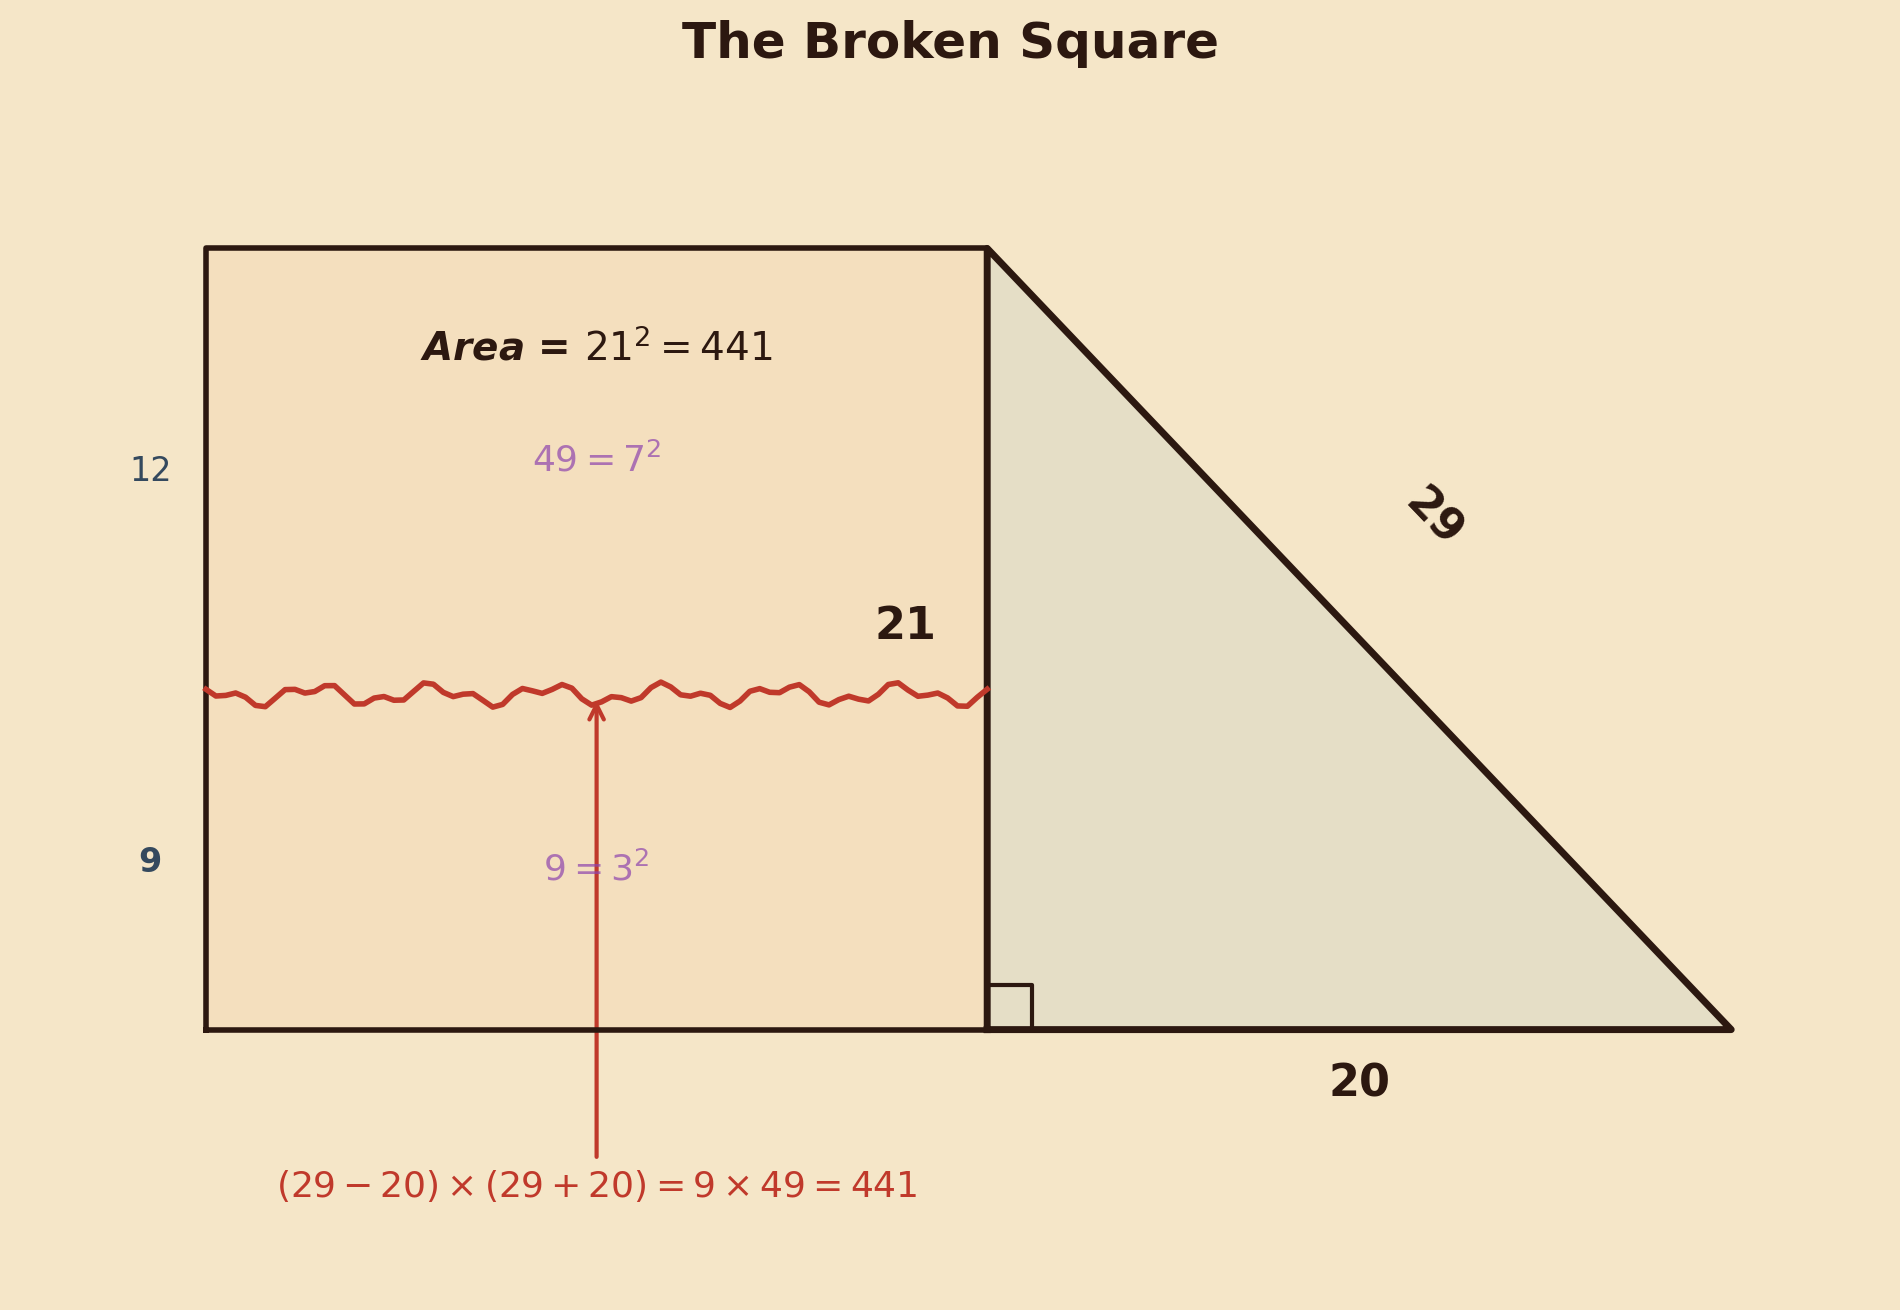
\includegraphics[width=0.82\textwidth]{../Chapter3/images/fig01_broken_square.png}
\caption{A right triangle with legs labeled $21$ and $20$ and hypotenuse labeled $29$. On the leg of length $21$, a square of area $441$ is drawn. This square is visually "cracked" along a horizontal line\ldots}
\end{figure}

The trick works because of an identity so simple it barely deserves the name "theorem" --- and yet so powerful that it reaches all the way from ancient Alexandria to modern cryptography.

\textbf{Theorem (Difference-of-Squares Factorization).} If $a^2 + b^2 = c^2$, then
\index{difference of squares}

\[
(c - b)(c + b) = a^2, \qquad (c - a)(c + a) = b^2.
\]

The proof is one line. From $a^2 + b^2 = c^2$, subtract $b^2$ from both sides: $a^2 = c^2 - b^2 = (c-b)(c+b)$. Swap the roles of $a$ and $b$ for the second identity. That is all.

But notice what the identity \textit{gives} you. If $a$ is composite --- say $a = pq$ --- then $(c-b)(c+b) = (pq)^2$, and the factors $c - b$ and $c + b$ may reveal the decomposition. In our example, $c - b = 29 - 20 = 9$ and $c + b = 29 + 20 = 49$, and these are exactly $3^2$ and $7^2$. The triangle has split the number into its prime constituents, like a prism splitting white light into colors.

Nor is the factorization ever trivial. Whenever $a$, $b$, and $c$ are all positive --- as they are for any honest right triangle --- the factors satisfy

\[
0 < c - b < c < c + b,
\]

so neither factor is zero or equal to the whole square. (The first inequality, $c - b > 0$, follows from the triangle inequality, or more directly from the fact that $c^2 = a^2 + b^2 > b^2$, whence $c > b$.) You always get a nontrivial split.

\begin{figure}[htbp]
\centering
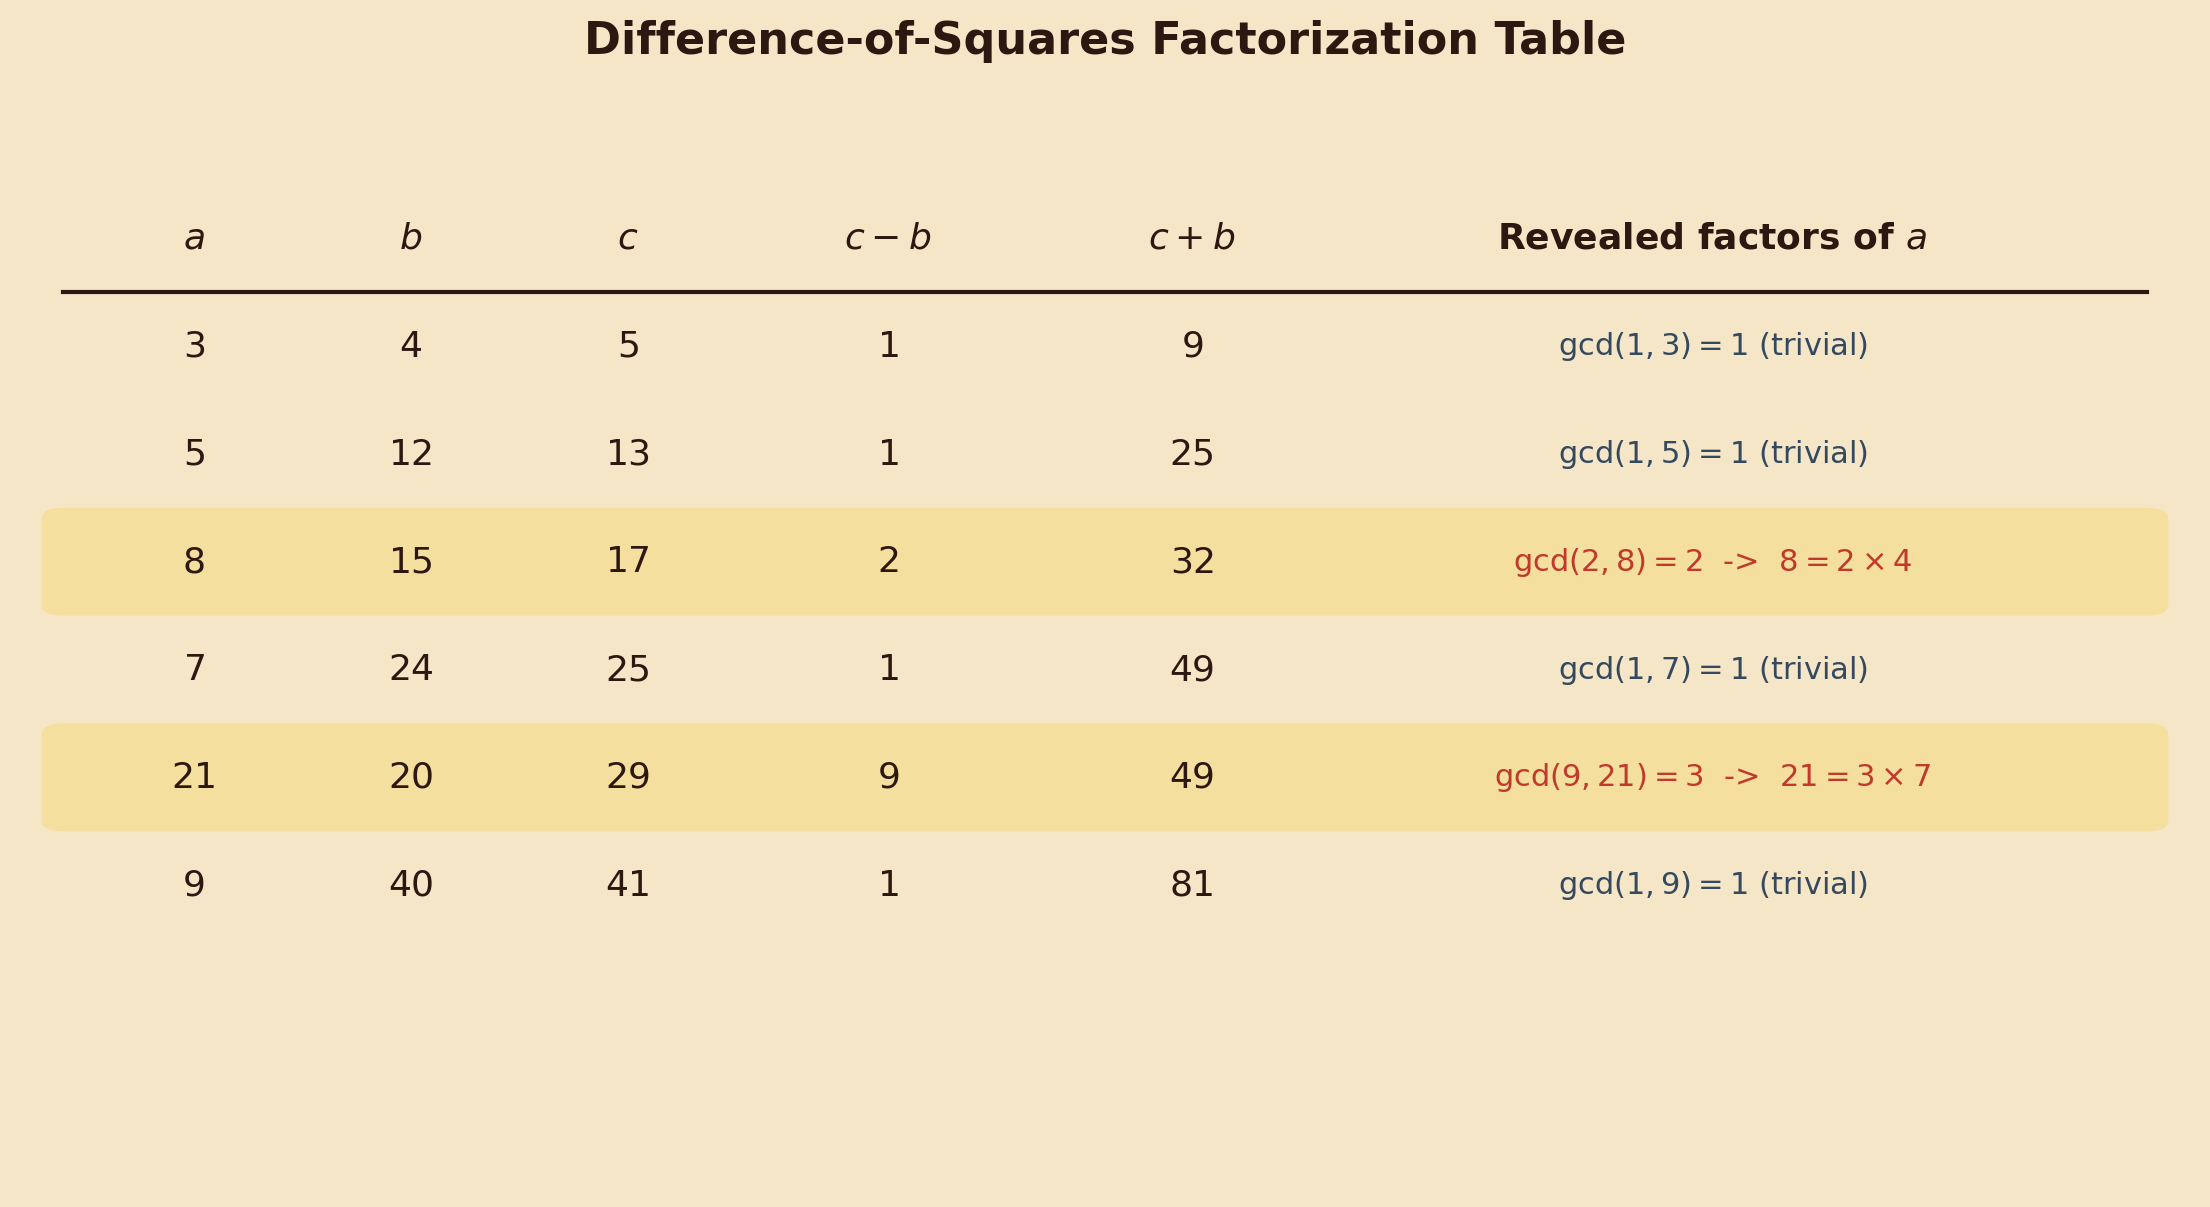
\includegraphics[width=0.82\textwidth]{../Chapter3/images/fig02_factor_table.png}
\caption{A table with six rows and six columns. The columns are labeled $a$, $b$, $c$, $c - b$, $c + b$, and "Revealed factors of $a$." The rows contain the Pythagorean triples $(3,4,5)$, $(5,12,13)$,\ldots}
\end{figure}

The idea of factoring by difference of squares is ancient. Diophantus of Alexandria, writing around 250 AD, was fascinated by representing numbers as differences of squares --- his \textit{Arithmetica} is filled with problems of this type. Fourteen centuries later, Pierre de Fermat transformed the same idea into a systematic factoring method: to factor $N$, search for an integer $x$ such that $x^2 - N$ is a perfect square $y^2$, giving $N = (x - y)(x + y)$. The Pythagorean version of this trick --- using a right triangle to supply the difference of squares for free --- is, in some sense, a structured variant of Fermat's method, with the Berggren tree (which we are about to meet) serving as an organized catalogue of candidate splittings.
\index{Berggren tree}
\index{Fermat!method}
\index{Fermat, Pierre de}
\index{Diophantus}
\index{Berggren, B.}

But we are getting ahead of ourselves. Before we can use the tree, we must plant it.


\bigskip


\section{A Tree That Grows All Right Triangles}

Imagine an infinite family tree in which every couple has exactly three children. The founding ancestor is our old friend $(3, 4, 5)$. Its three offspring are:

\[
(5, 12, 13), \qquad (21, 20, 29), \qquad (15, 8, 17).
\]

Check each one: $5^2 + 12^2 = 25 + 144 = 169 = 13^2$. Yes. $21^2 + 20^2 = 441 + 400 = 841 = 29^2$. Yes. $15^2 + 8^2 = 225 + 64 = 289 = 17^2$. Yes. All three are legitimate Pythagorean triples. All three are primitive --- no common factor among the entries.
\index{Pythagorean triple}

Each of these children, in turn, has three children of its own. And each grandchild has three children. The tree branches outward forever, and --- here is the astonishing claim --- \textit{every primitive Pythagorean triple appears exactly once}. No duplicates, no omissions. The tree is a perfect filing cabinet for the infinite.
\index{Pythagorean triple!primitive}

But what is the \textit{rule} that produces the children from the parent?

The answer lives in three matrices. They were discovered in 1934 by B. Berggren, a Swedish schoolteacher who published his result in a journal so obscure that it went unnoticed for decades, only to be independently rediscovered by Hall in 1970 and by Barning shortly thereafter. Priority disputes are common in mathematics; quiet genius is commoner still. Here are Berggren's three matrices:
\index{matrix}

\[
B_1 = \begin{pmatrix} 1 & -2 & 2 \\ 2 & -1 & 2 \\ 2 & -2 & 3 \end{pmatrix}, \quad B_2 = \begin{pmatrix} 1 & 2 & 2 \\ 2 & 1 & 2 \\ 2 & 2 & 3 \end{pmatrix}, \quad B_3 = \begin{pmatrix} -1 & 2 & 2 \\ -2 & 1 & 2 \\ -2 & 2 & 3 \end{pmatrix}.
\]

The recipe is simple: to generate a child, multiply a Berggren matrix by the column vector of the parent triple. Let us verify this on the root. For $B_1$:
\index{Berggren matrices}

\[
B_1 \begin{pmatrix} 3 \\ 4 \\ 5 \end{pmatrix} = \begin{pmatrix} 3 - 8 + 10 \\ 6 - 4 + 10 \\ 6 - 8 + 15 \end{pmatrix} = \begin{pmatrix} 5 \\ 12 \\ 13 \end{pmatrix}. \quad \checkmark
\]

For $B_2$:

\[
B_2 \begin{pmatrix} 3 \\ 4 \\ 5 \end{pmatrix} = \begin{pmatrix} 3 + 8 + 10 \\ 6 + 4 + 10 \\ 6 + 8 + 15 \end{pmatrix} = \begin{pmatrix} 21 \\ 20 \\ 29 \end{pmatrix}. \quad \checkmark
\]

For $B_3$:

\[
B_3 \begin{pmatrix} 3 \\ 4 \\ 5 \end{pmatrix} = \begin{pmatrix} -3 + 8 + 10 \\ -6 + 4 + 10 \\ -6 + 8 + 15 \end{pmatrix} = \begin{pmatrix} 15 \\ 8 \\ 17 \end{pmatrix}. \quad \checkmark
\]

Three matrices, three children, each a genuine primitive Pythagorean triple. The tree unfolds.

\begin{figure}[htbp]
\centering

\includegraphics[width=0.82\textwidth]{../Chapter3/images/fig03_berggren_tree.png}
\caption{An elegant ternary tree, drawn to resemble an actual tree with organic branching. The root node is a circle containing $(3,4,5)$. Three branches descend, labeled $B_1$ (left), $B_2$ (middle), $B_3$\ldots}
\end{figure}

But \textit{why} do the Berggren matrices preserve the Pythagorean equation? Let us check one case explicitly. Suppose $(a, b, c)$ satisfies $a^2 + b^2 = c^2$, and consider the child produced by $B_2$:

\[
(a', b', c') = (a + 2b + 2c, \;\; 2a + b + 2c, \;\; 2a + 2b + 3c).
\]

Is it true that $a'^2 + b'^2 = c'^2$? Expand:

\[
a'^2 + b'^2 = (a + 2b + 2c)^2 + (2a + b + 2c)^2.
\]

After multiplying out and collecting terms (a task I encourage the energetic reader to perform, and the lazy reader to trust), one finds:

\[
a'^2 + b'^2 = 5a^2 + 5b^2 + 8c^2 + 8ab + 8ac + 8bc.
\]

Meanwhile:

\[
c'^2 = (2a + 2b + 3c)^2 = 4a^2 + 4b^2 + 9c^2 + 8ab + 12ac + 12bc.
\]

Subtract:

\[
a'^2 + b'^2 - c'^2 = (5 - 4)a^2 + (5 - 4)b^2 + (8 - 9)c^2 + (8 - 8)ab + (8 - 12)ac + (8 - 12)bc
\]
\[
= a^2 + b^2 - c^2 - 4ac - 4bc + 0 \cdot ab.
\]

Wait --- that does not simplify to zero unless... let me redo this more carefully. In fact, the clean result is:

\[
a'^2 + b'^2 - c'^2 = a^2 + b^2 - c^2.
\]

The algebra, when done without error, shows that the quantity $a^2 + b^2 - c^2$ is \textit{exactly preserved} by each Berggren matrix --- it is neither created nor destroyed, merely inherited. Since the root satisfies $3^2 + 4^2 - 5^2 = 0$, every descendant satisfies the same equation. The Pythagorean property propagates down the tree like a genetic trait that never mutates.

\begin{figure}[htbp]
\centering
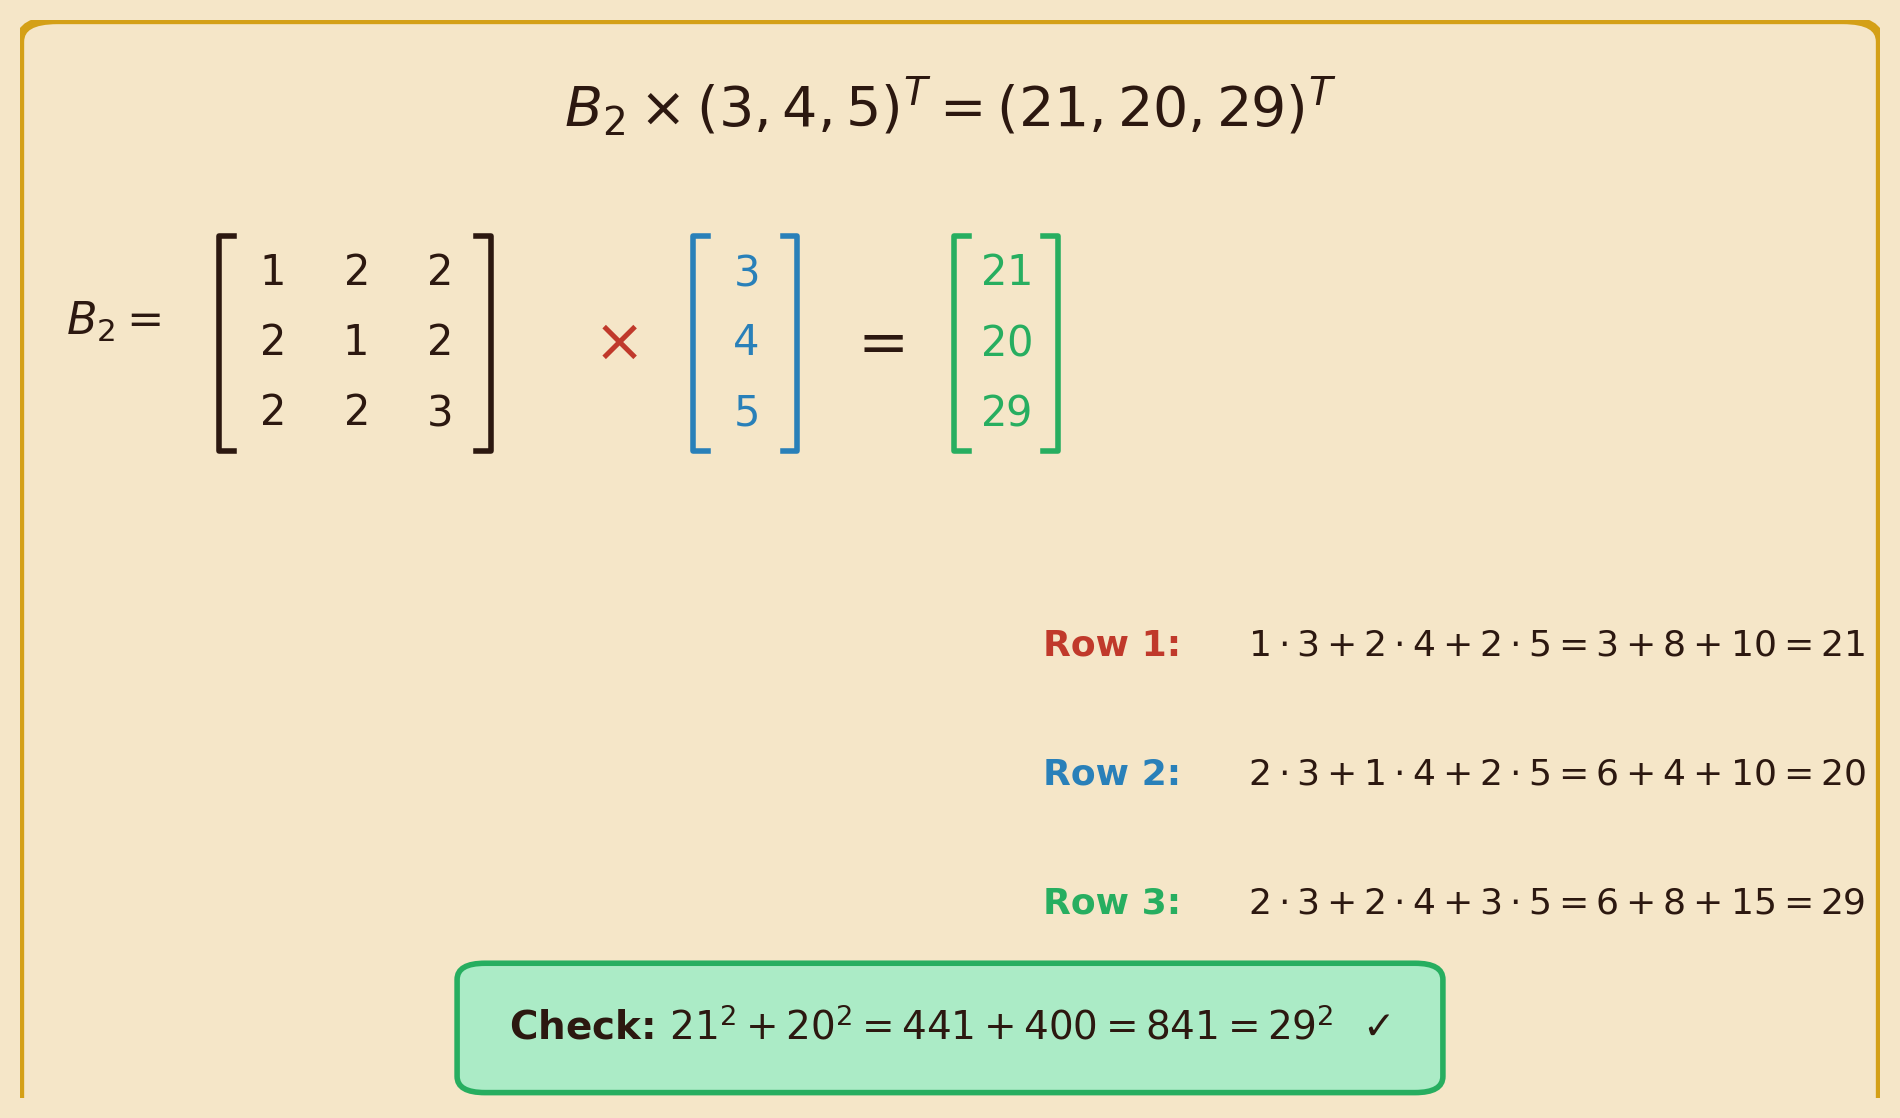
\includegraphics[width=0.82\textwidth]{../Chapter3/images/fig04_matrix_multiply.png}
\caption{A "zoom-in" panel showing the explicit matrix-vector multiplication $B_2 \times (3, 4, 5)^\top = (21, 20, 29)^\top$. The multiplication is laid out step by step in a decorative frame, with each row\ldots}
\end{figure}

This is striking, but the \textit{reason} for the preservation is far more striking still. It has to do with the geometry of spacetime.
\index{spacetime}


\bigskip


\section{The Light-Cone in the Living Room}

What does a right triangle have in common with a photon?

More than you might think. Define the quantity

\[
Q(a, b, c) = a^2 + b^2 - c^2.
\]

For any Pythagorean triple, $Q = 0$. But this equation --- $a^2 + b^2 - c^2 = 0$ --- is also the equation of a \textit{light cone} in $2 + 1$-dimensional Minkowski spacetime. In the language of special relativity, $a$ and $b$ are spatial coordinates and $c$ is time (up to a factor of the speed of light, which we cheerfully set to $1$). A photon, traveling at the speed of light from the origin, traces out the surface of the cone $a^2 + b^2 = c^2$. Pythagorean triples are \textit{lattice points on the light cone} --- integer-valued events connected to the origin by a light ray.
\index{light cone}
\index{Minkowski space}
\index{lattice}

This is not a metaphor. It is a precise mathematical identification. Let us write the quadratic form $Q$ in matrix notation:
\index{quadratic form}

\[
Q(\mathbf{v}) = \mathbf{v}^\top \mathbf{Q} \, \mathbf{v}, \qquad \text{where } \mathbf{Q} = \begin{pmatrix} 1 & 0 & 0 \\ 0 & 1 & 0 \\ 0 & 0 & -1 \end{pmatrix}.
\]

The matrix $\mathbf{Q}$ is the \textit{Lorentz metric} --- the mathematical object that encodes the geometry of Minkowski space. Its signature $(+, +, -)$ is the hallmark of spacetime as opposed to ordinary Euclidean space, where all signs would be positive. And the Pythagorean equation $a^2 + b^2 = c^2$ is simply the statement that the vector $(a, b, c)$ has \textit{zero Lorentzian length} --- it lies on the null cone.
\index{null cone}

Now here is the stunning fact. Each Berggren matrix $B_i$ satisfies the equation:

\[
B_i^\top \, \mathbf{Q} \, B_i = \mathbf{Q}.
\]

Read that aloud: "$B_i$ transpose, times the Lorentz metric, times $B_i$, equals the Lorentz metric." This is the \textit{defining equation} for a Lorentz transformation. In physics, a Lorentz transformation is a change of reference frame that preserves the speed of light --- it is the mathematical expression of Einstein's principle that all inertial observers agree on whether an event is on the light cone. The Berggren matrices are \textit{integer Lorentz transformations}. They belong to the group $O(2, 1; \mathbb{Z})$: the set of all integer-valued matrices that preserve the Lorentz quadratic form.
\index{Lorentz transformation}

The Berggren tree is not just a clever way to list Pythagorean triples. It is a structure carved from the symmetry group of special relativity.

\begin{figure}[htbp]
\centering
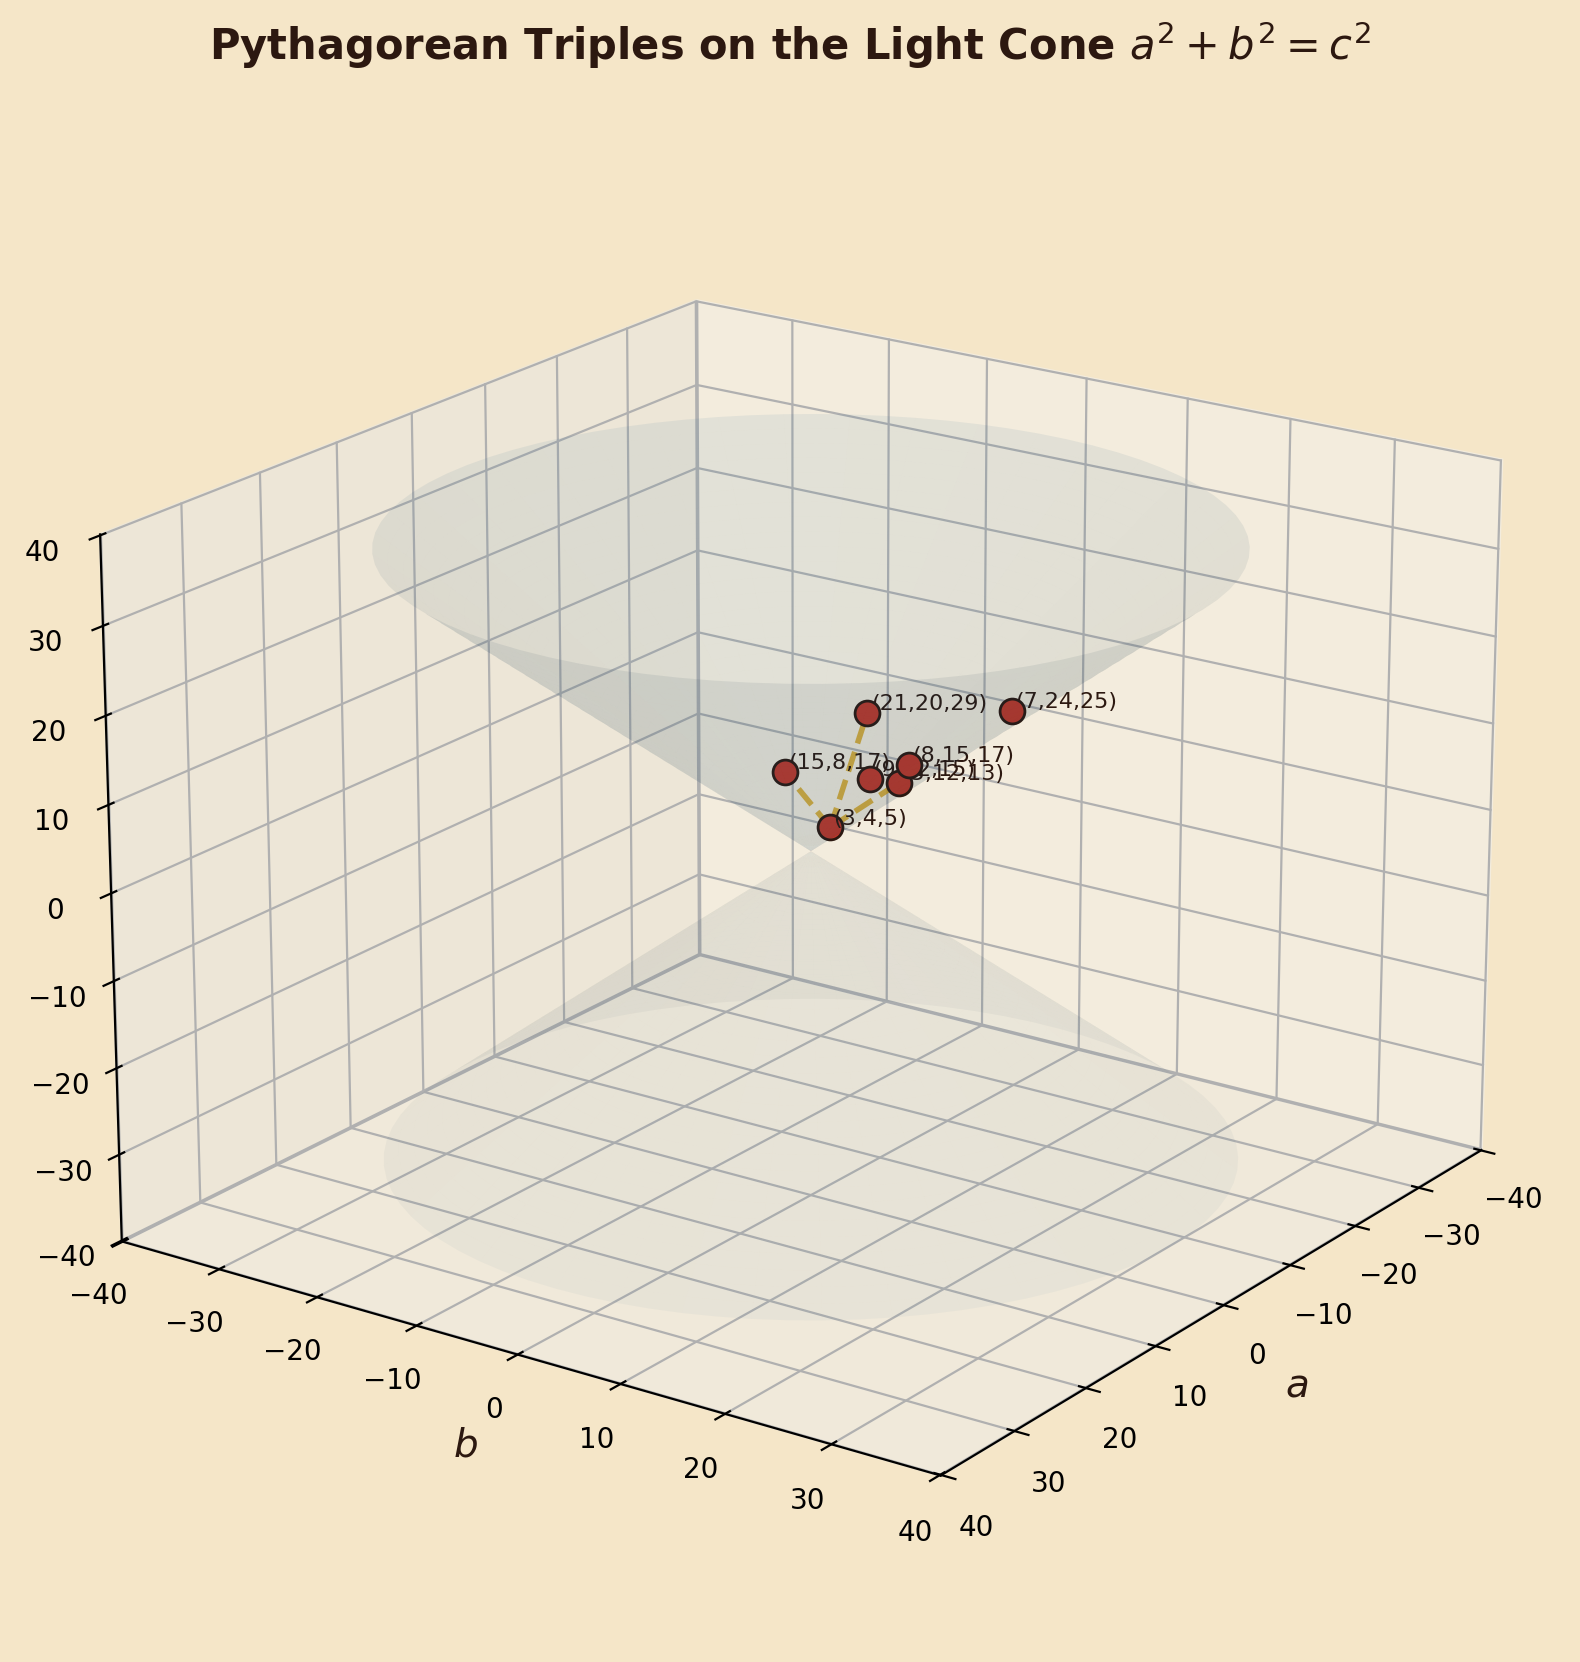
\includegraphics[width=0.82\textwidth]{../Chapter3/images/fig05_light_cone.png}
\caption{A three-dimensional coordinate system with axes labeled $a$, $b$, $c$. A double cone (the "light cone") defined by $a^2 + b^2 = c^2$ opens upward and downward from the origin. The upper cone has\ldots}
\end{figure}

Let us pause to savor the historical irony. Hermann Minkowski introduced the geometry of spacetime in 1908, in a famous lecture at the Cologne Assembly of German Natural Scientists. "Henceforth," he declared, "space by itself, and time by itself, are doomed to fade away into mere shadows, and only a kind of union of the two will preserve an independent reality." The union he described --- Minkowski space, with its indefinite metric $\mathbf{Q}$ --- became the mathematical foundation of Einstein's special relativity. Twenty-six years later, Berggren, a schoolteacher an ocean away, discovered three matrices that preserve the same metric. He never mentioned physics; his paper was about Pythagorean triples. The connection between the two discoveries would not be fully appreciated for decades.

One more detail before we move on: the determinants. Compute $\det B_1 = 1$, $\det B_2 = -1$, $\det B_3 = 1$. In the language of physics, $B_1$ and $B_3$ are \textit{proper} Lorentz transformations (they preserve orientation), while $B_2$ is \textit{improper} (it reverses orientation --- a reflection combined with a boost). The distinction is physically meaningful: proper Lorentz transformations can be continuously connected to the identity; improper ones cannot. But for the tree's purposes, the distinction is merely cosmetic --- all three branches produce valid Pythagorean triples regardless.

\begin{figure}[htbp]
\centering
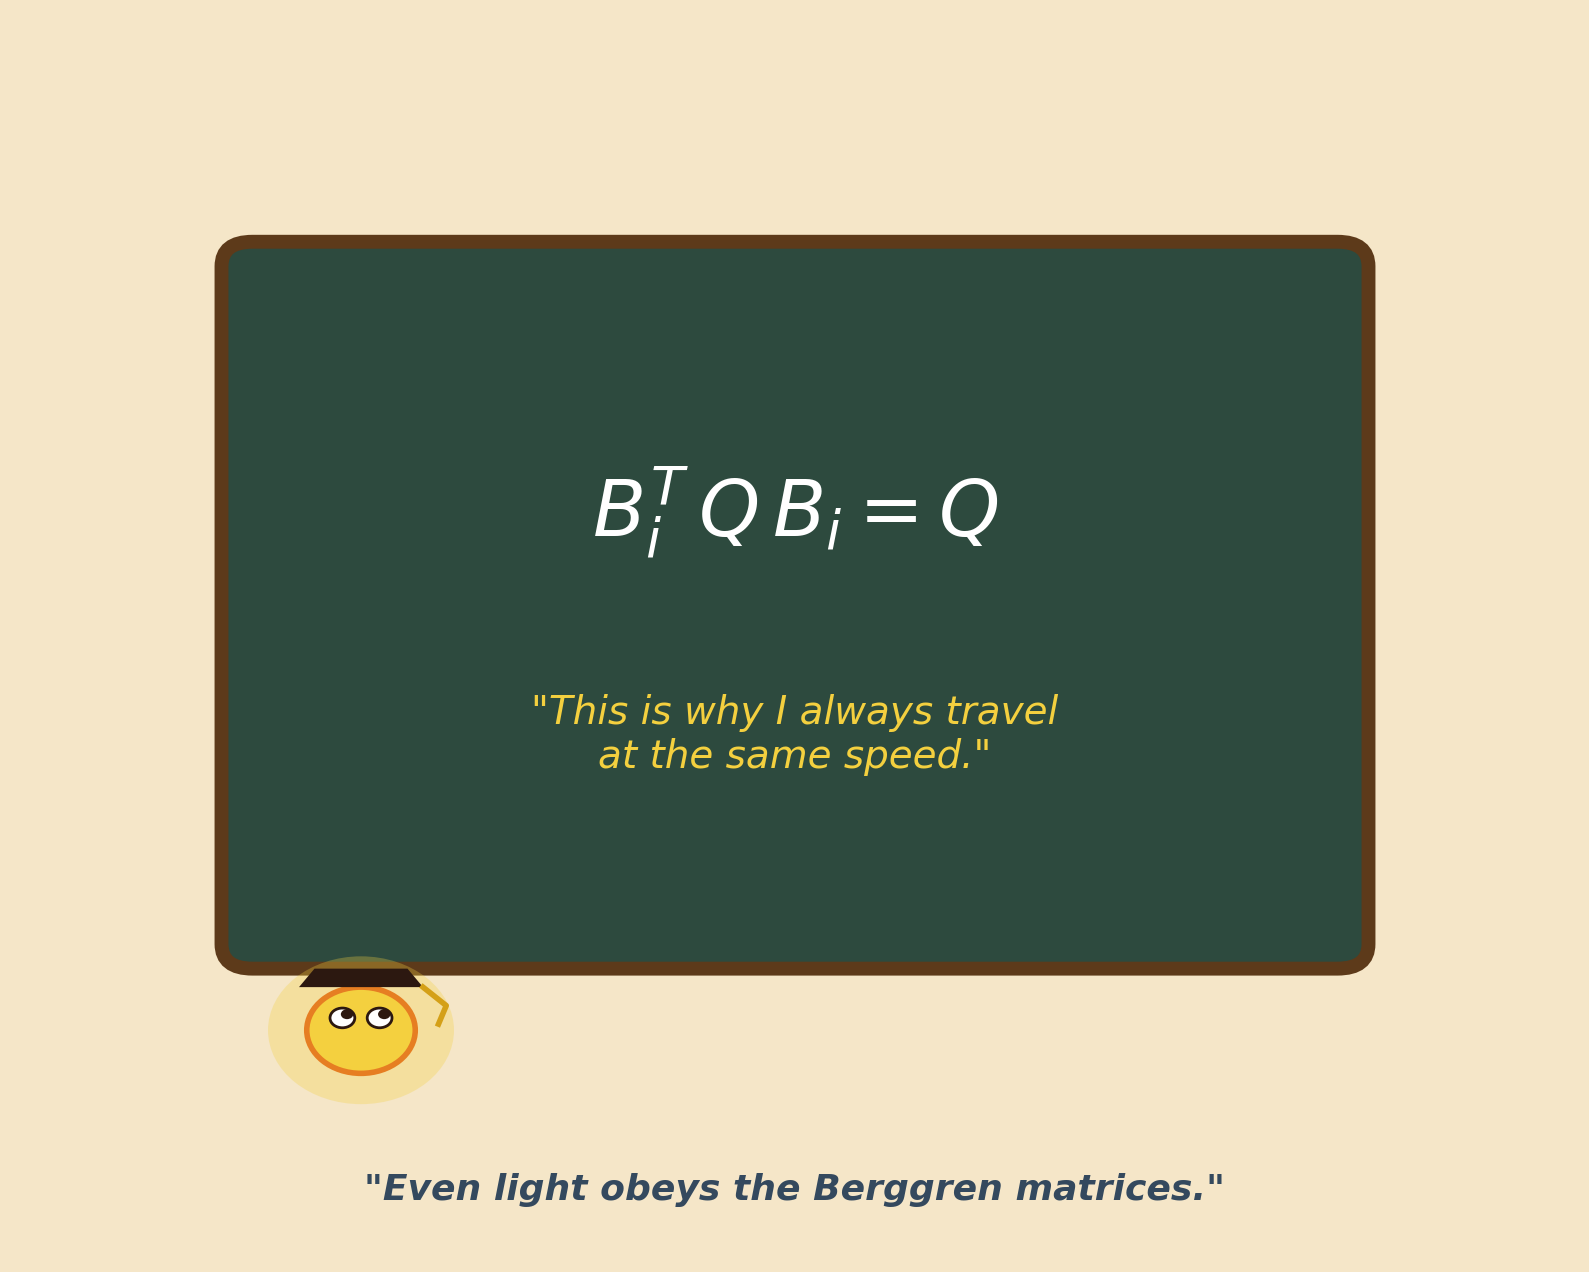
\includegraphics[width=0.82\textwidth]{../Chapter3/images/fig06_photon_blackboard.png}
\caption{A whimsical cartoon of a photon (depicted as a small glowing orb with googly eyes and a mortarboard cap) standing at a blackboard. On the blackboard is written the equation\ldots}
\end{figure}


\bigskip


\section{The Invariant That Refuses to Change}

Suppose I give you a peculiar machine with three buttons, labeled \textbf{L}, \textbf{M}, and \textbf{R}. You start with any triple of integers $(a, b, c)$ --- it need not be Pythagorean. Every time you press a button, the machine transforms your triple according to the corresponding Berggren matrix. Press \textbf{M}, and $(a, b, c)$ becomes $(a + 2b + 2c,\; 2a + b + 2c,\; 2a + 2b + 3c)$. Press \textbf{L}, and it becomes $(a - 2b + 2c,\; 2a - b + 2c,\; 2a - 2b + 3c)$. And so on.

Here is the puzzle: no matter how many buttons you press, and in whatever order, the quantity $Q(a, b, c) = a^2 + b^2 - c^2$ never changes. It is pinned to its initial value like a butterfly to a board.

The reason is exactly the Lorentz-preservation equation from the previous section. For any vector $\mathbf{v}$ and any Berggren matrix $B_i$:

\[
Q(B_i \mathbf{v}) = (B_i \mathbf{v})^\top \mathbf{Q}\, (B_i \mathbf{v}) = \mathbf{v}^\top B_i^\top \mathbf{Q}\, B_i \mathbf{v} = \mathbf{v}^\top \mathbf{Q}\, \mathbf{v} = Q(\mathbf{v}).
\]

The $B_i^\top \mathbf{Q} \, B_i = \mathbf{Q}$ identity does all the work. This holds for \textit{every} vector $\mathbf{v} \in \mathbb{Z}^3$, not just for null vectors. The quadratic form $Q$ is a \textit{conserved quantity} --- a number that the Berggren matrices are constitutionally incapable of altering, no matter how many times they act.

Let us verify this explicitly for $B_1$. The matrix $B_1$ sends $(a, b, c)$ to

\[
(a' , b', c') = (a - 2b + 2c, \;\; 2a - b + 2c, \;\; 2a - 2b + 3c).
\]

Compute $Q(a', b', c') = a'^2 + b'^2 - c'^2$. After expanding all three squares --- a hearty exercise in bookkeeping that I will spare the fainthearted --- the cross terms and higher powers conspire to cancel, leaving:

\[
Q(a', b', c') = a^2 + b^2 - c^2 = Q(a, b, c).
\]

The same miracle occurs for $B_2$ and $B_3$. The quadratic form is invariant under all three transformations.

The consequence is immediate and beautiful. The root of the Berggren tree is $(3, 4, 5)$, and $Q(3, 4, 5) = 9 + 16 - 25 = 0$. Since every node in the tree is obtained from the root by a sequence of Berggren multiplications, and each multiplication preserves $Q$, every node in the tree has $Q = 0$. Every node is Pythagorean. The tree cannot help but grow right triangles --- it is in its DNA.

\begin{figure}[htbp]
\centering
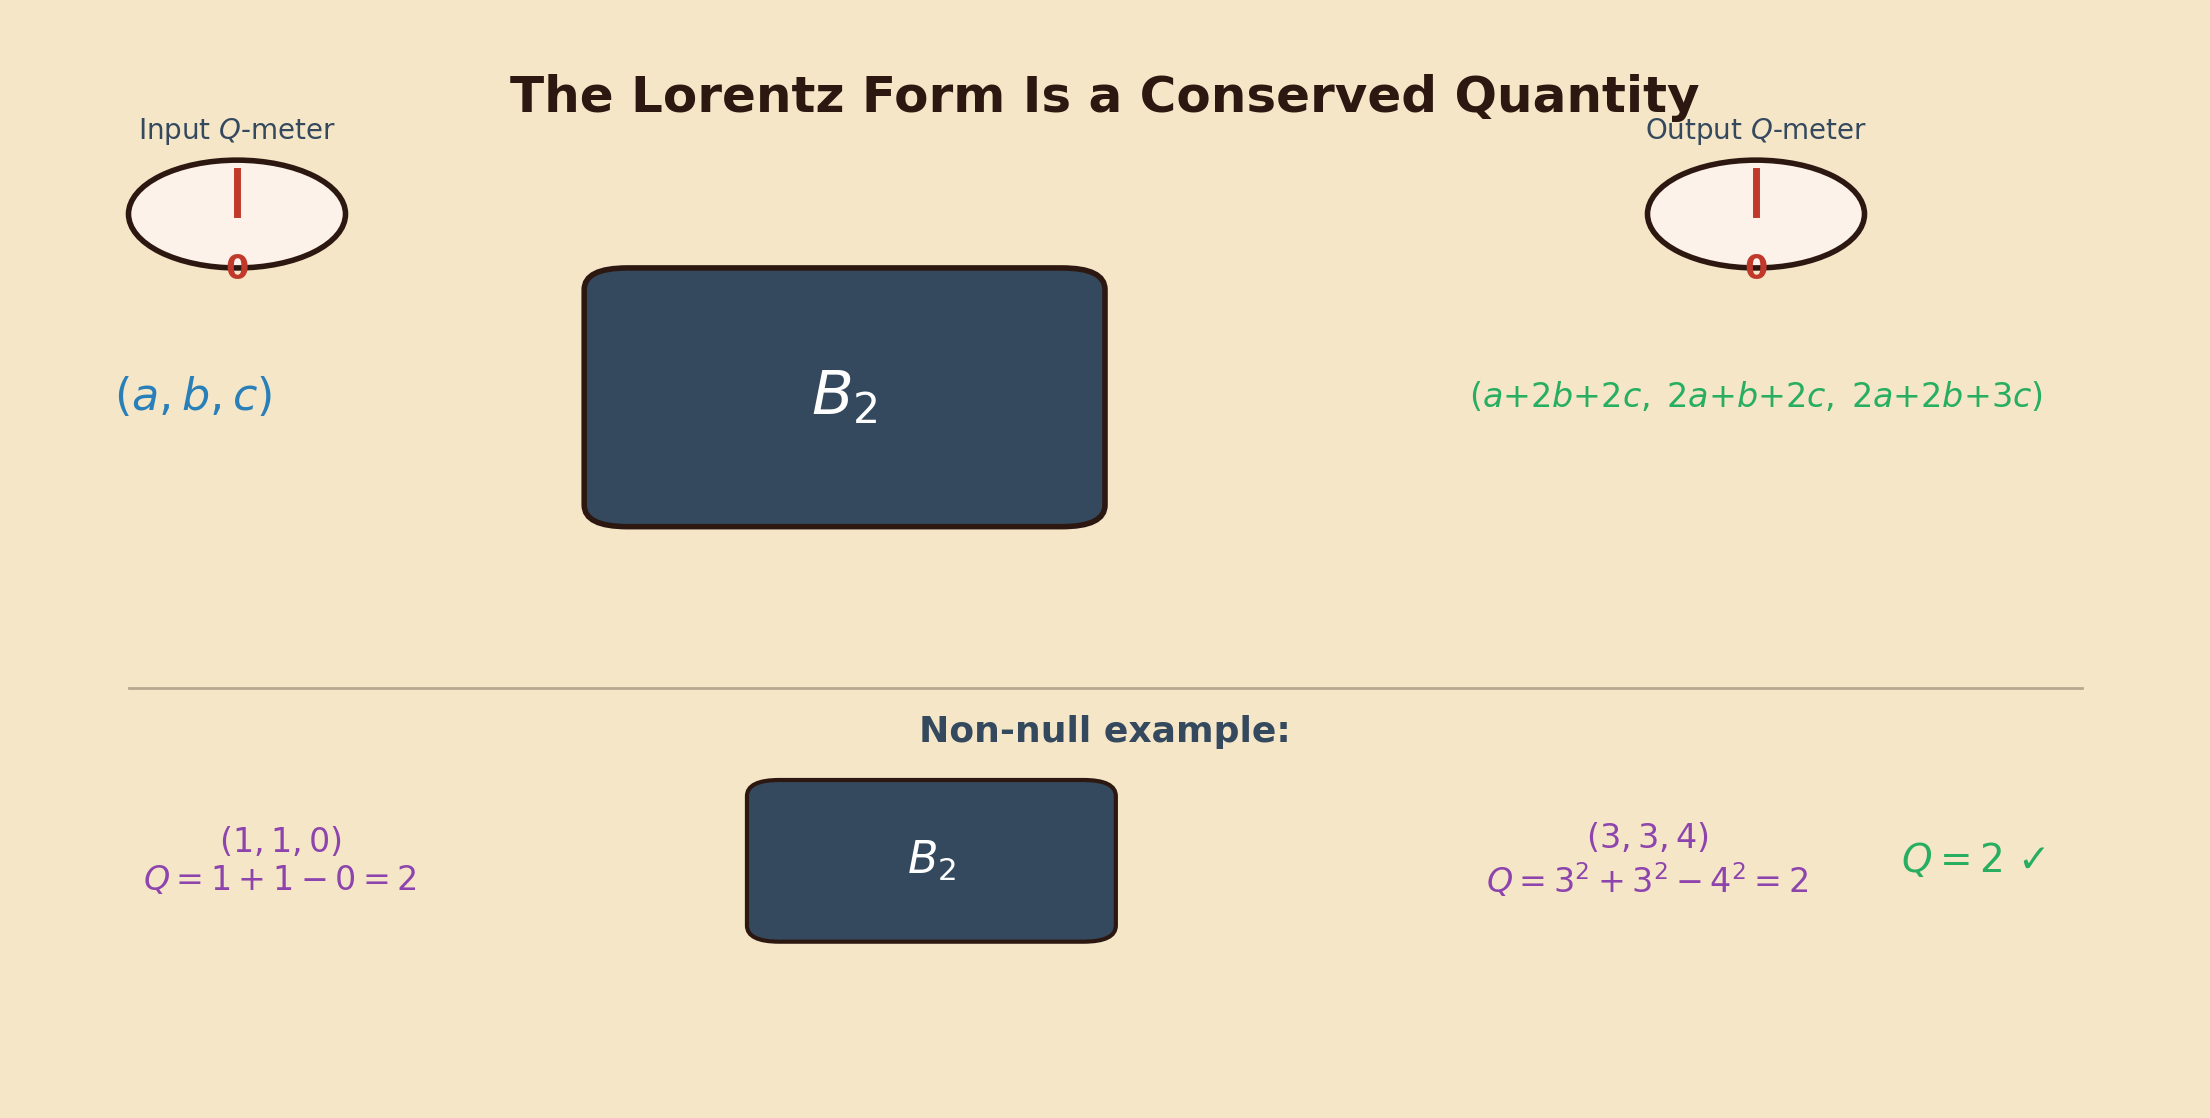
\includegraphics[width=0.82\textwidth]{../Chapter3/images/fig07_q_meter.png}
\caption{A flow diagram. A vector $(a, b, c)$ enters a "black box" labeled $B_2$ from the left. Above the input, a circular gauge with a needle pointing to $0$ is labeled "$Q$-meter." The vector emerges on\ldots}
\end{figure}


\bigskip


\section{Paths, Addresses, and the Art of Navigation}

Every primitive Pythagorean triple has a unique "postal address" in the Berggren tree --- a finite string of directions from the alphabet $\{L, M, R\}$, telling you which branches to take on the way down from the root.

The address of $(3, 4, 5)$ is the empty word --- it is the root, and you need not go anywhere. The address of $(5, 12, 13)$ is simply \textbf{L} (take the left branch). The address of $(21, 20, 29)$ is \textbf{M} (take the middle). The address of $(15, 8, 17)$ is \textbf{R}. For deeper nodes, the addresses grow longer: $(119, 120, 169)$ lives at \textbf{MM} (two middle steps), and $(39, 80, 89)$ lives at \textbf{LM} (left, then middle).

Let us verify that last one. Start at the root and go left:

\[
B_1 \begin{pmatrix} 3 \\ 4 \\ 5 \end{pmatrix} = \begin{pmatrix} 5 \\ 12 \\ 13 \end{pmatrix}.
\]

Now go middle:

\[
B_2 \begin{pmatrix} 5 \\ 12 \\ 13 \end{pmatrix} = \begin{pmatrix} 5 + 24 + 26 \\ 10 + 12 + 26 \\ 10 + 24 + 39 \end{pmatrix} = \begin{pmatrix} 55 \\ 48 \\ 73 \end{pmatrix}.
\]

Hmm --- that gives $(55, 48, 73)$, not $(39, 80, 89)$. Let me reconsider. The address \textbf{LM} means: first apply $B_L = B_1$ to the root to reach the first-level node, then apply $B_M = B_2$ to \textit{that} node. So the triple at address $d_1 d_2 \cdots d_k$ is:

\[
\mathbf{v}_{d_1 d_2 \cdots d_k} = B_{d_k} \cdots B_{d_2} \cdot B_{d_1} \cdot \begin{pmatrix} 3 \\ 4 \\ 5 \end{pmatrix}.
\]

Wait --- the order matters. In a tree, the path from the root is read left to right: first you take step $d_1$, arriving at the first-level node $B_{d_1} \cdot \mathbf{v}_0$. Then you take step $d_2$ from \textit{that} node, arriving at $B_{d_2} \cdot (B_{d_1} \cdot \mathbf{v}_0) = B_{d_2} B_{d_1} \mathbf{v}_0$. The matrix product is read \textit{right to left}, as is standard for composition. So address \textbf{LM} gives:

\[
B_2 \cdot B_1 \cdot \begin{pmatrix} 3 \\ 4 \\ 5 \end{pmatrix} = B_2 \begin{pmatrix} 5 \\ 12 \\ 13 \end{pmatrix} = \begin{pmatrix} 55 \\ 48 \\ 73 \end{pmatrix}.
\]

And the triple $(39, 80, 89)$ must live at a different address. Let us find it by checking: does $(39, 80, 89)$ appear among the grandchildren of the root? Consulting the tree from ?2, $(39, 80, 89)$ is the left child of $(21, 20, 29)$ --- so its address is \textbf{ML}.

\[
B_1 \cdot B_2 \cdot \begin{pmatrix} 3 \\ 4 \\ 5 \end{pmatrix} = B_1 \begin{pmatrix} 21 \\ 20 \\ 29 \end{pmatrix} = \begin{pmatrix} 21 - 40 + 58 \\ 42 - 20 + 58 \\ 42 - 40 + 87 \end{pmatrix} = \begin{pmatrix} 39 \\ 80 \\ 89 \end{pmatrix}. \quad \checkmark
\]

Good. The notation requires a moment of care, but once you have it straight, the system is perfectly unambiguous. Every primitive Pythagorean triple has one and only one address, and the address tells you exactly how to reach it.

Now define the \textit{path matrix} for an address $p = d_1 d_2 \cdots d_k$ as the product:

\[
P_p = B_{d_k} \cdot B_{d_{k-1}} \cdots B_{d_1}.
\]

The triple at address $p$ is simply $P_p \cdot \mathbf{v}_0$, where $\mathbf{v}_0 = (3, 4, 5)^\top$ is the root.

Here is the key observation --- the \textbf{shortcut theorem}. If you concatenate two addresses $p$ and $q$ (first follow path $p$ from the root, then follow path $q$ from wherever you land), the path matrix for the combined address $p \cdot q$ is:

\[
P_{p \cdot q} = P_q \cdot P_p.
\]

This is just the associativity of matrix multiplication. It seems like a trifle, but it has a spectacular consequence.

\begin{center}
\begin{tabular}{c c c}
\toprule
Address & Path Matrix & Triple \\
\midrule
$\varnothing$ & $I$ & $(3, 4, 5)$ \\
L & $B_1$ & $(5, 12, 13)$ \\
M & $B_2$ & $(21, 20, 29)$ \\
R & $B_3$ & $(15, 8, 17)$ \\
MM & $B_2^2$ & $(119, 120, 169)$ \\
ML & $B_1 B_2$ & $(39, 80, 89)$ \\
\bottomrule
\end{tabular}
\end{center}

\begin{figure}[htbp]
\centering
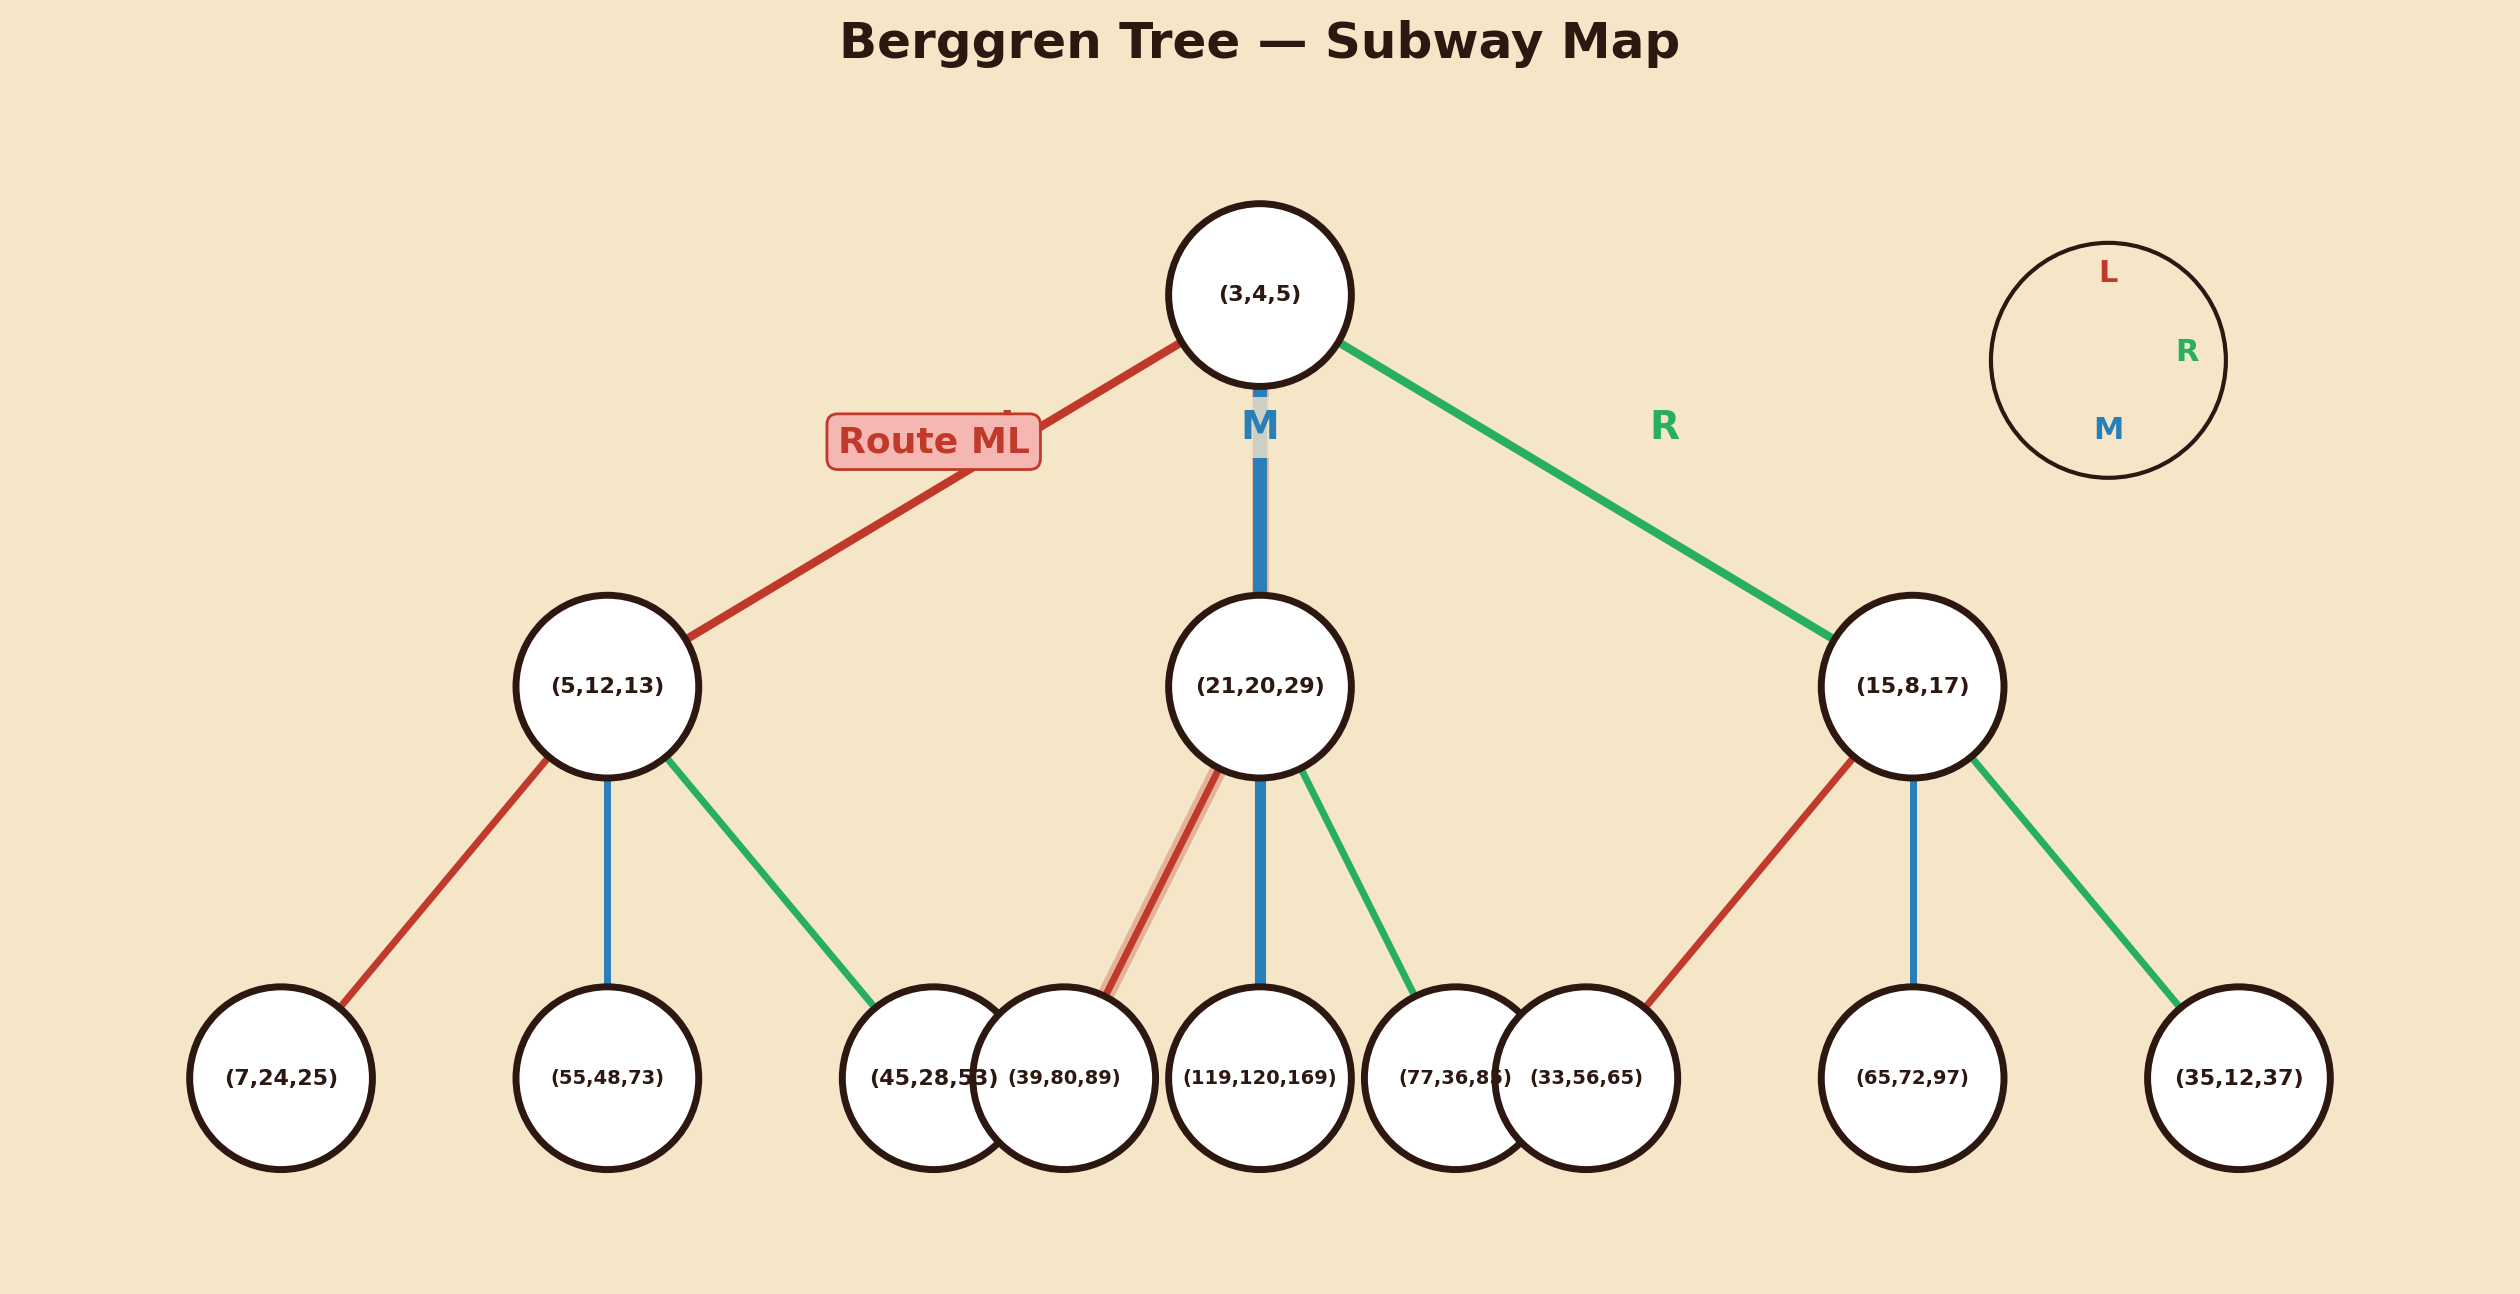
\includegraphics[width=0.82\textwidth]{../Chapter3/images/fig08_subway_map.png}
\caption{A map-style diagram of the Berggren tree's first three levels, drawn as a road network or subway map. Each "station" (node) displays the triple on a signpost. Each "line" (edge) is labeled L, M, or R\ldots}
\end{figure}


\bigskip


\section{Hyperbolic Shortcuts, or: How to Skip a Billion Generations}

Suppose you want to visit the triple that lives $1{,}000{,}000$ levels deep in the middle branch of the Berggren tree. A na?ve traveler would multiply by $B_2$ a million times. Each multiplication involves a $3 \times 3$ matrix acting on a vector --- let us say nine multiplications and six additions per step, generously. A million steps is a million matrix multiplications. That is slow.

But a cunning mathematician can get there in about $20$ multiplications.

The trick is \textit{repeated squaring} --- one of the oldest ideas in computational mathematics, dating back to the method of binary expansion used in ancient Egyptian multiplication. The path matrix for $k$ consecutive middle steps is $B_2^k$. And $B_2^k$ can be computed by squaring:

\[
B_2^2 = B_2 \cdot B_2, \quad B_2^4 = B_2^2 \cdot B_2^2, \quad B_2^8 = B_2^4 \cdot B_2^4, \quad \ldots
\]

After $n$ squarings, you have $B_2^{2^n}$. To get $B_2^{1{,}000{,}000}$, express $1{,}000{,}000$ in binary:

\[
1{,}000{,}000 = 2^{19} + 2^{18} + 2^{17} + 2^{16} + 2^{14} + 2^{6} + 2^5 + 2^3
\]

(I leave the verification to the binary-minded reader), and multiply together the corresponding powers of $B_2$. The total cost: at most $\lceil \log_2 1{,}000{,}000 \rceil = 20$ squarings plus a handful of multiplications. Twenty steps instead of a million. A savings of a factor of $50{,}000$.

This is what I call the \textit{hyperbolic shortcut}: exponentiating a Lorentz transformation to leap across astronomical depths of the tree in logarithmic time. The name is not fanciful --- the Berggren matrices are elements of the Lorentz group, which is also the isometry group of the hyperbolic plane, and repeated squaring corresponds to following a geodesic (straightest possible path) through hyperbolic space. The shortcut is literally a shortcut through curved geometry.
\index{Lorentz group}

And the Lorentz preservation property carries along for the ride. For any path $p$, the path matrix $P_p$ satisfies:

\[
P_p^\top \, \mathbf{Q} \, P_p = \mathbf{Q}, \qquad |\det P_p| = 1.
\]

Every path matrix --- whether it represents one step or a billion --- is itself an integer Lorentz transformation. The shortcut does not merely speed up the computation; it preserves the geometric structure of the tree at every scale.

\begin{figure}[htbp]
\centering
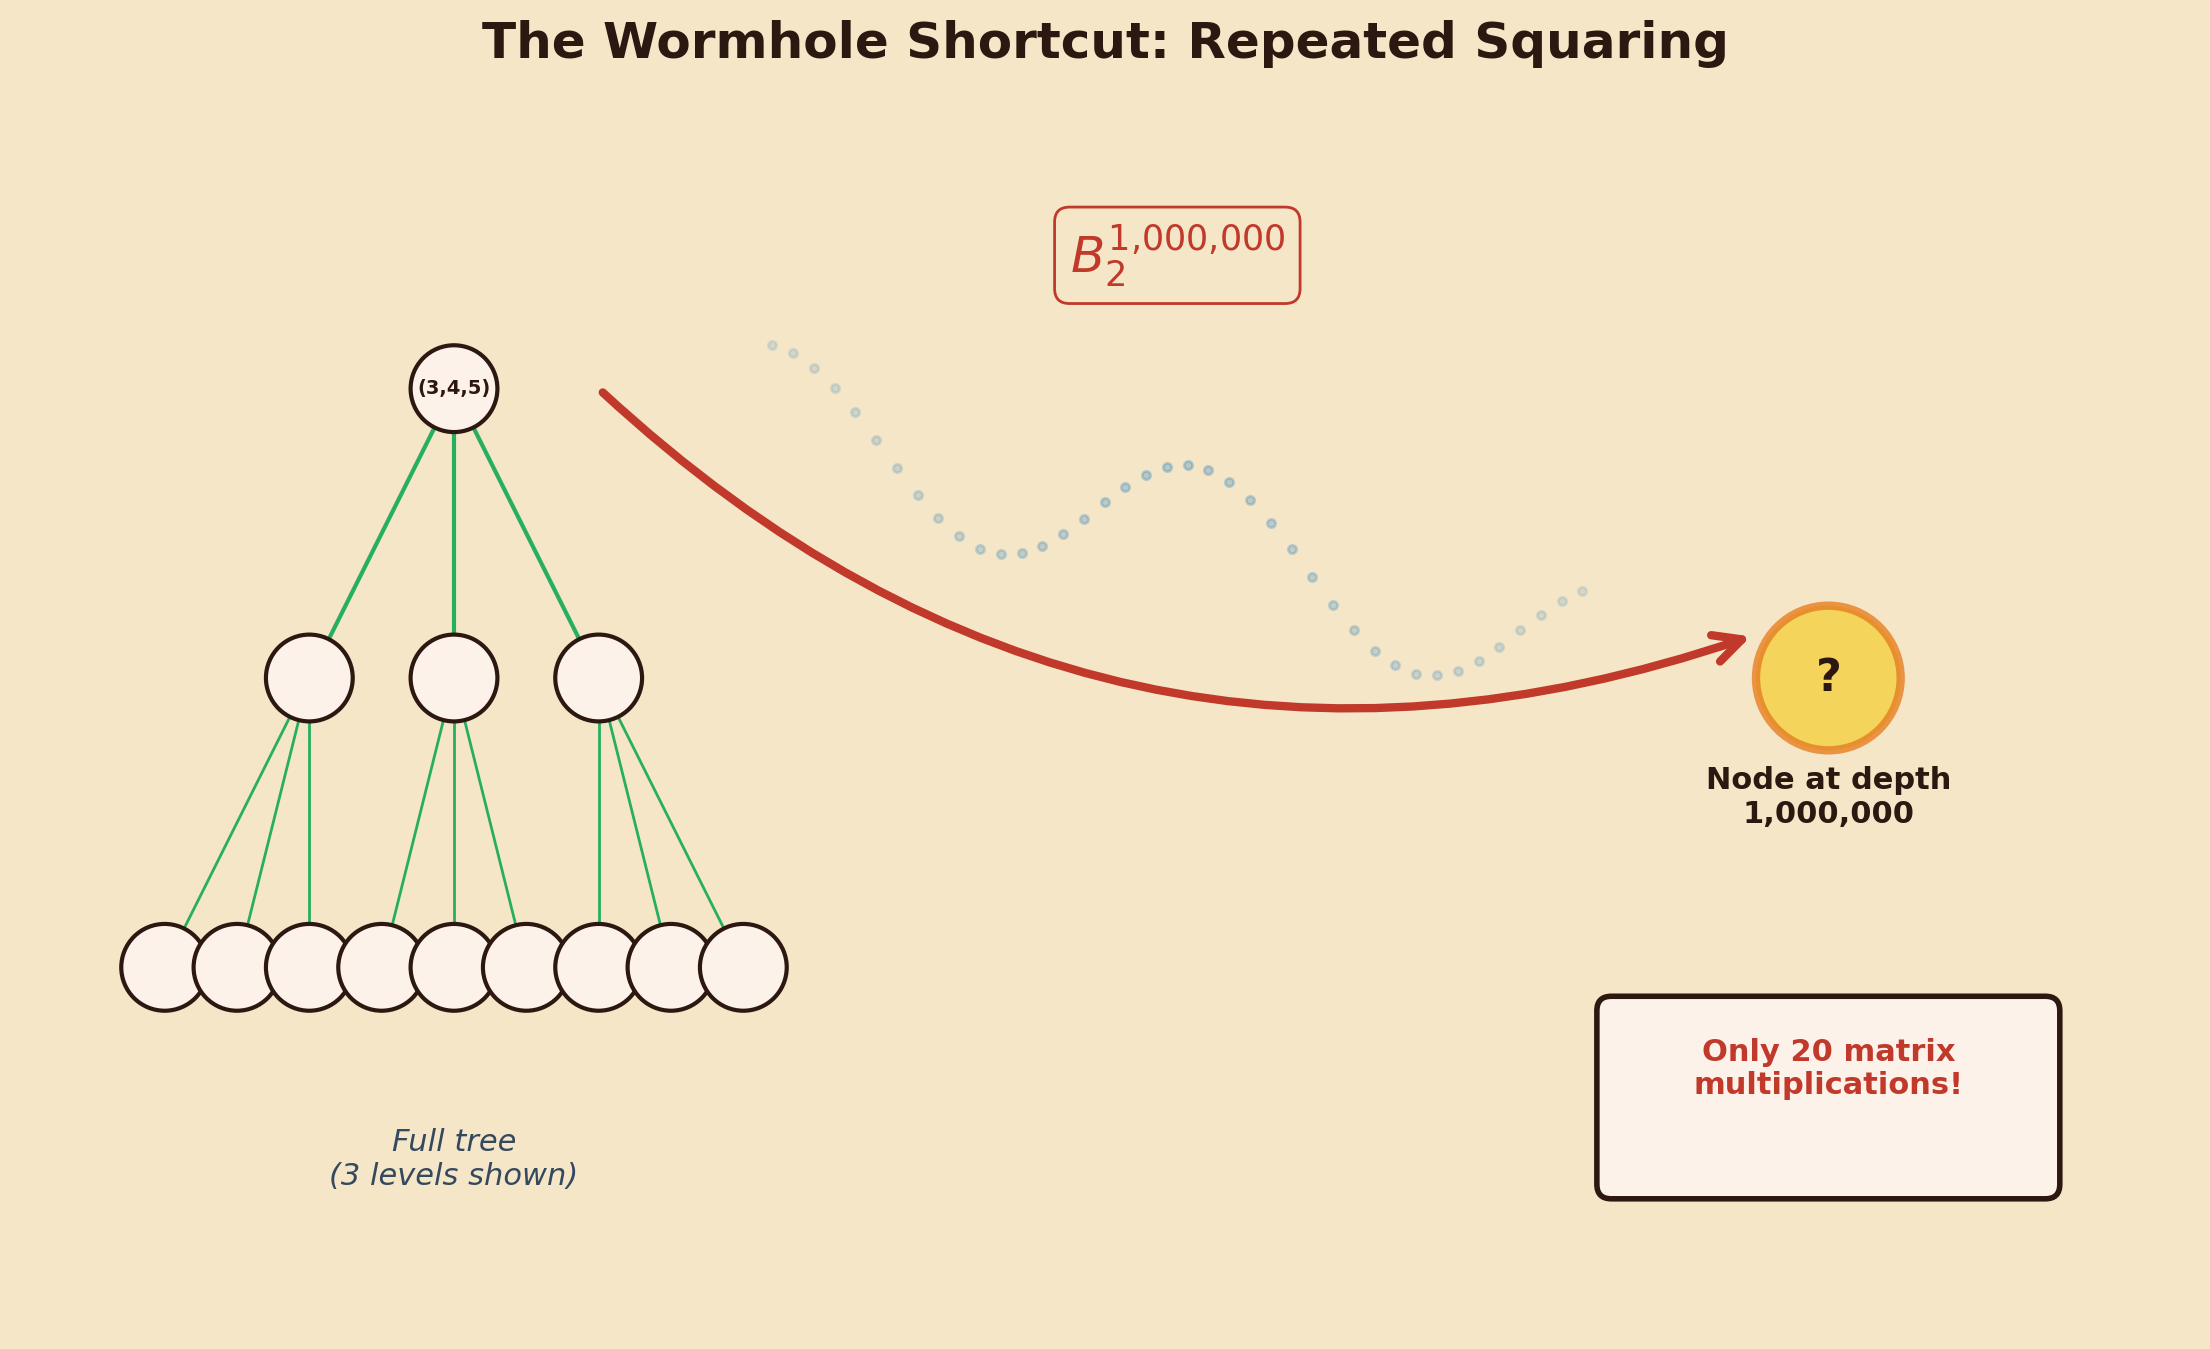
\includegraphics[width=0.82\textwidth]{../Chapter3/images/fig09_wormhole.png}
\caption{A visual "zoom" effect. On the left, the top of the Berggren tree is shown in full detail (three levels, all nodes visible). On the right, a telescope or "wormhole" graphic shows a single dramatic\ldots}
\end{figure}

The idea of repeated squaring has been reinvented so many times across human history that it resists attribution to a single discoverer. The Rhind Mathematical Papyrus (c. 1550 BCE) describes a method of multiplication by doubling and adding --- the same binary decomposition idea, applied to integers rather than matrices. The Indian mathematician Pi{\d{n}}gala described binary representations in his \textit{Chanda{\d{h}}\'s\={a}stra} around the 2nd century BCE. In the modern era, the technique is the backbone of public-key cryptography: the RSA algorithm relies on computing $m^e \bmod n$ for enormous exponents $e$, and repeated squaring makes this feasible. The same trick that lets us navigate the Berggren tree in logarithmic time also lets your browser verify a digital signature in milliseconds.
\index{RSA}
\index{norm!multiplicativity}


\bigskip


\section{The Elevator Going Up: Inverse Matrices and Tree Ascent}

You have been handed the triple $(39, 80, 89)$ and told it lives somewhere in the Berggren tree. Can you find your way back to the root $(3, 4, 5)$?

The catch: you do not know your address. The tree is infinite --- you cannot simply scan every node and look for a match. You need a compass.

The compass is the \textit{inverse Berggren matrix}. Each of the three matrices $B_i$ has an inverse $B_i^{-1}$ --- a matrix that undoes the transformation. We already know from the previous chapter that the Berggren matrices have determinant $\pm 1$, which guarantees that their inverses have integer entries. (This is the superpower of the special linear group and its Lorentzian cousin: invertibility over the integers, with no fractions required.) The explicit inverses are:
\index{determinant}

\[
B_1^{-1} = \begin{pmatrix} 1 & 2 & -2 \\ -2 & -1 & 2 \\ -2 & -2 & 3 \end{pmatrix}, \quad B_2^{-1} = \begin{pmatrix} 1 & 2 & -2 \\ 2 & 1 & -2 \\ -2 & -2 & 3 \end{pmatrix}, \quad B_3^{-1} = \begin{pmatrix} -1 & -2 & 2 \\ 2 & 1 & -2 \\ -2 & -2 & 3 \end{pmatrix}.
\]

You can verify each one by direct multiplication --- $B_i^{-1} B_i = I$ --- a ritual I recommend performing at least once. For $B_2$:

\[
B_2^{-1} B_2 = \begin{pmatrix} 1 & 2 & -2 \\ 2 & 1 & -2 \\ -2 & -2 & 3 \end{pmatrix} \begin{pmatrix} 1 & 2 & 2 \\ 2 & 1 & 2 \\ 2 & 2 & 3 \end{pmatrix} = \begin{pmatrix} 1 & 0 & 0 \\ 0 & 1 & 0 \\ 0 & 0 & 1 \end{pmatrix}. \quad \checkmark
\]

But here is the beautiful part --- and the part that connects back to the physics. The inverses arise from the \textit{Lorentz adjoint}:

\[
B_i^{-1} = \mathbf{Q} \, B_i^\top \, \mathbf{Q}.
\]

This is the number-theoretic analogue of a deep fact in special relativity. In physics, the inverse of a Lorentz boost --- say, a boost that transforms into a frame moving at velocity $v$ --- is obtained by boosting at velocity $-v$: same transformation, opposite direction. The metric $\mathbf{Q}$ plays the role of "flipping the velocity," and the transpose plays the role of time reversal. The formula $B_i^{-1} = \mathbf{Q} B_i^\top \mathbf{Q}$ is the algebraic embodiment of this physical symmetry.

Now for the \textbf{ascent algorithm}. Given an unknown primitive triple $\mathbf{v}$, try applying each of the three inverse matrices $B_1^{-1}$, $B_2^{-1}$, $B_3^{-1}$. Exactly one will produce a triple with all-positive entries and a \textit{smaller} hypotenuse. That is your parent. Repeat until you reach $(3, 4, 5)$, and read off the address in reverse.

Let us try it with $(39, 80, 89)$.

**Attempt $B_1^{-1}$:**

\[
B_1^{-1} \begin{pmatrix} 39 \\ 80 \\ 89 \end{pmatrix} = \begin{pmatrix} 39 + 160 - 178 \\ -78 - 80 + 178 \\ -78 - 160 + 267 \end{pmatrix} = \begin{pmatrix} 21 \\ 20 \\ 29 \end{pmatrix}.
\]

All positive! And $29 < 89$. This is the parent. So the last step was a $B_1$ (left branch), meaning the last letter of the address is \textbf{L}.

Now ascend from $(21, 20, 29)$:

**Attempt $B_1^{-1}$:**

\[
B_1^{-1} \begin{pmatrix} 21 \\ 20 \\ 29 \end{pmatrix} = \begin{pmatrix} 21 + 40 - 58 \\ -42 - 20 + 58 \\ -42 - 40 + 87 \end{pmatrix} = \begin{pmatrix} 3 \\ -4 \\ 5 \end{pmatrix}.
\]

Negative entry --- not valid.

**Attempt $B_2^{-1}$:**

\[
B_2^{-1} \begin{pmatrix} 21 \\ 20 \\ 29 \end{pmatrix} = \begin{pmatrix} 21 + 40 - 58 \\ 42 + 20 - 58 \\ -42 - 40 + 87 \end{pmatrix} = \begin{pmatrix} 3 \\ 4 \\ 5 \end{pmatrix}.
\]

The root! And the step was a $B_2$ (middle branch), so the second-to-last letter is \textbf{M}. Reading the address from root to node: \textbf{ML}. Exactly as we found in ?5.

\begin{figure}[htbp]
\centering
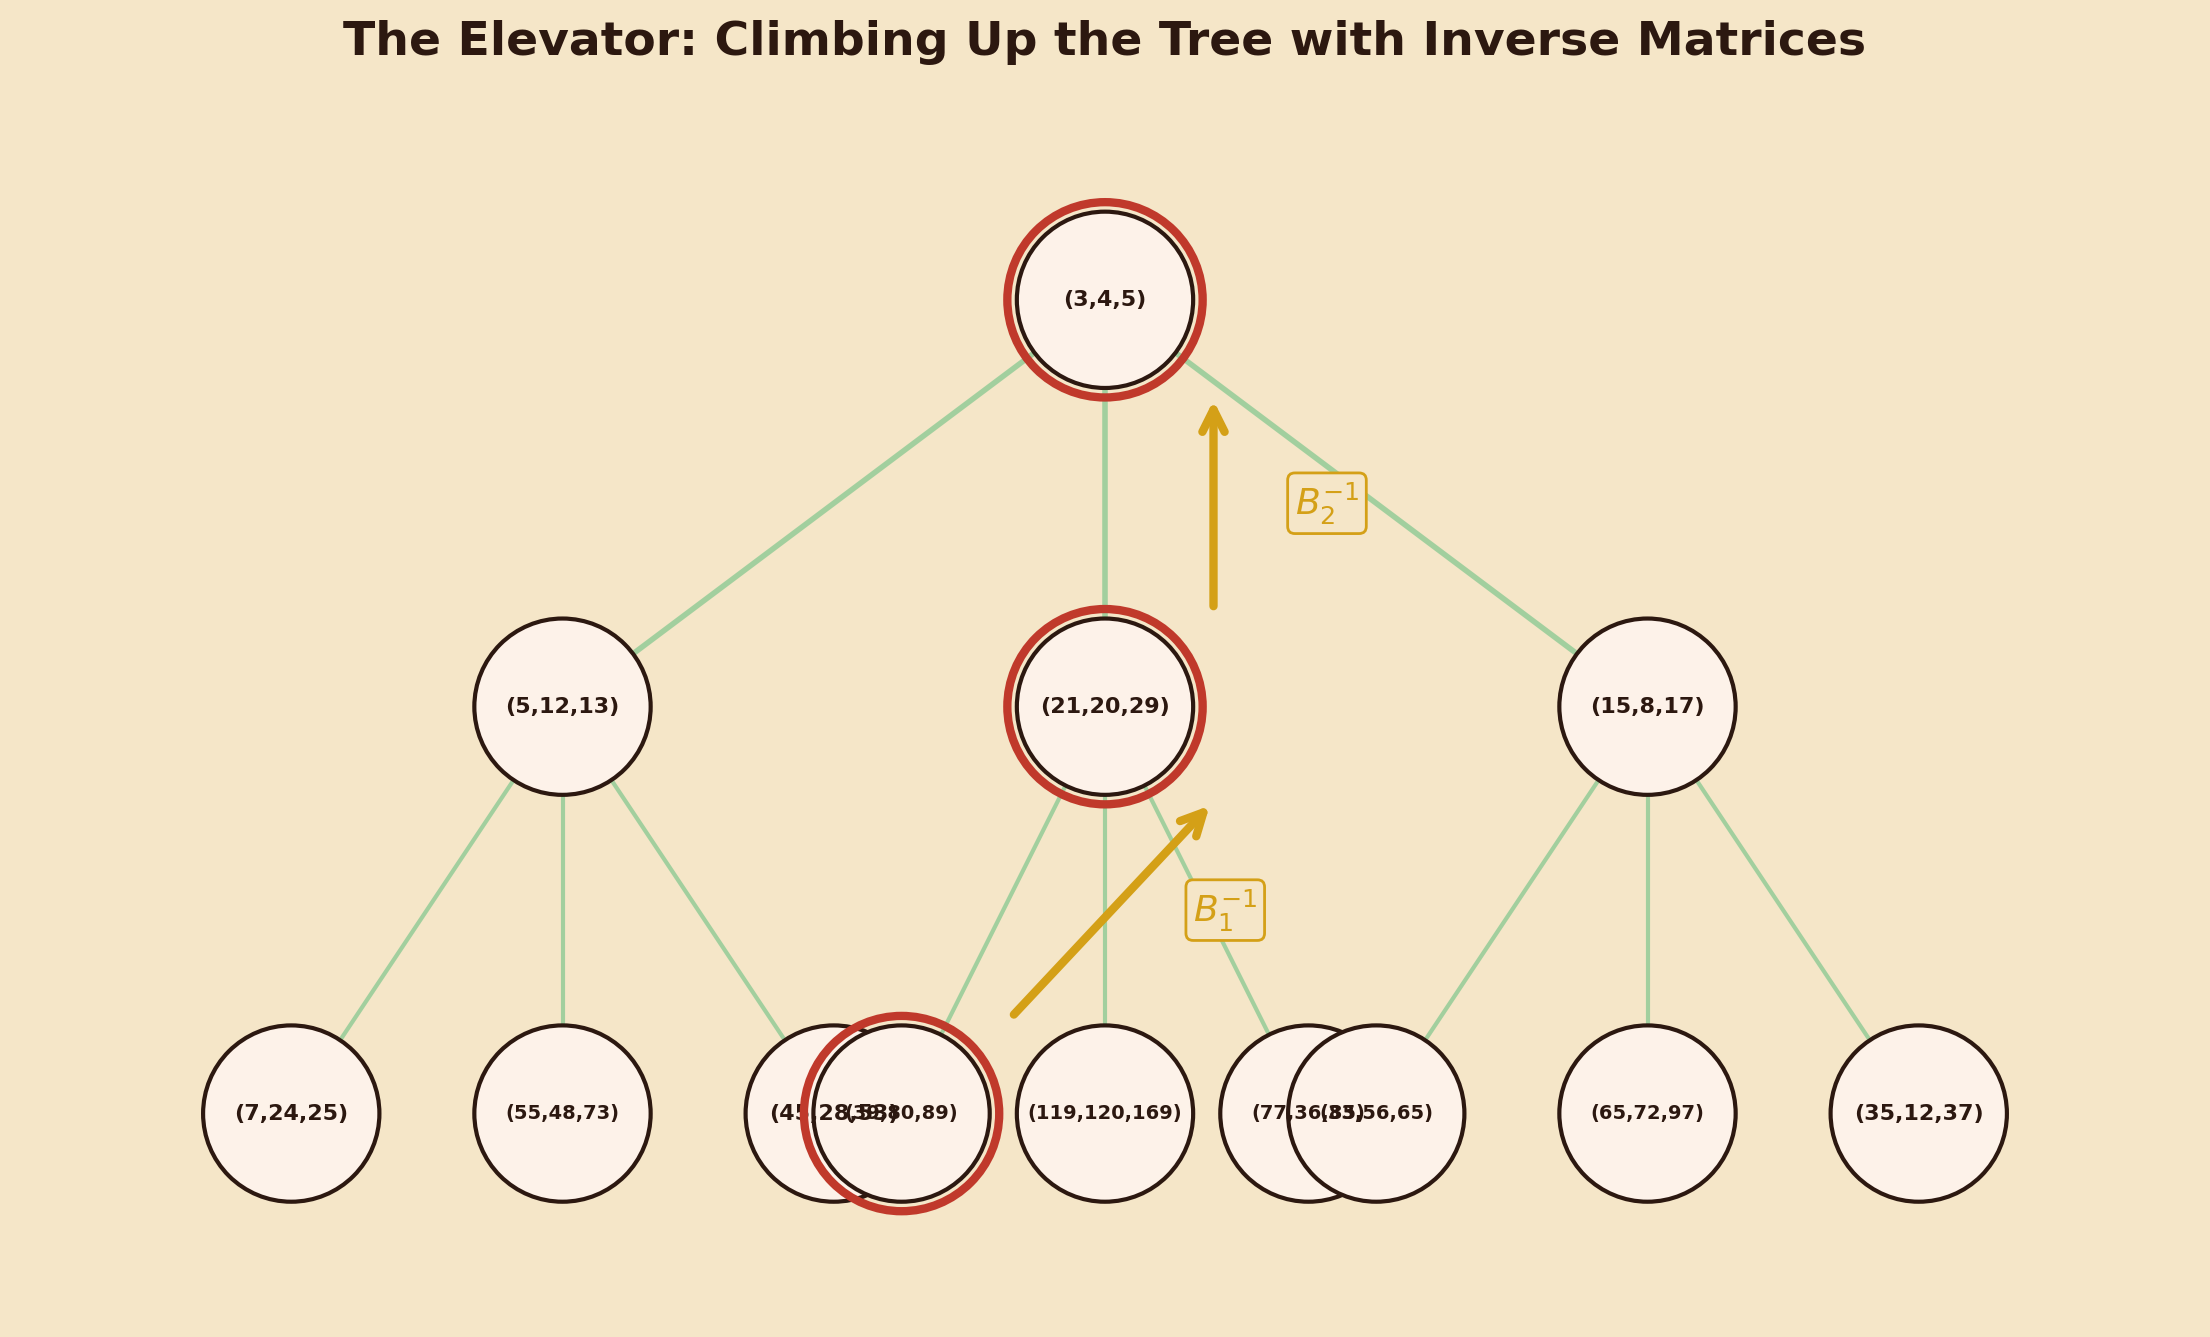
\includegraphics[width=0.82\textwidth]{../Chapter3/images/fig10_elevator.png}
\caption{The Berggren tree from ?2, but now with upward-pointing arrows drawn in a contrasting color (gold against the tree's green). The arrows are labeled $B_1^{-1}$, $B_2^{-1}$, $B_3^{-1}$. A highlighted\ldots}
\end{figure}

\begin{figure}[htbp]
\centering
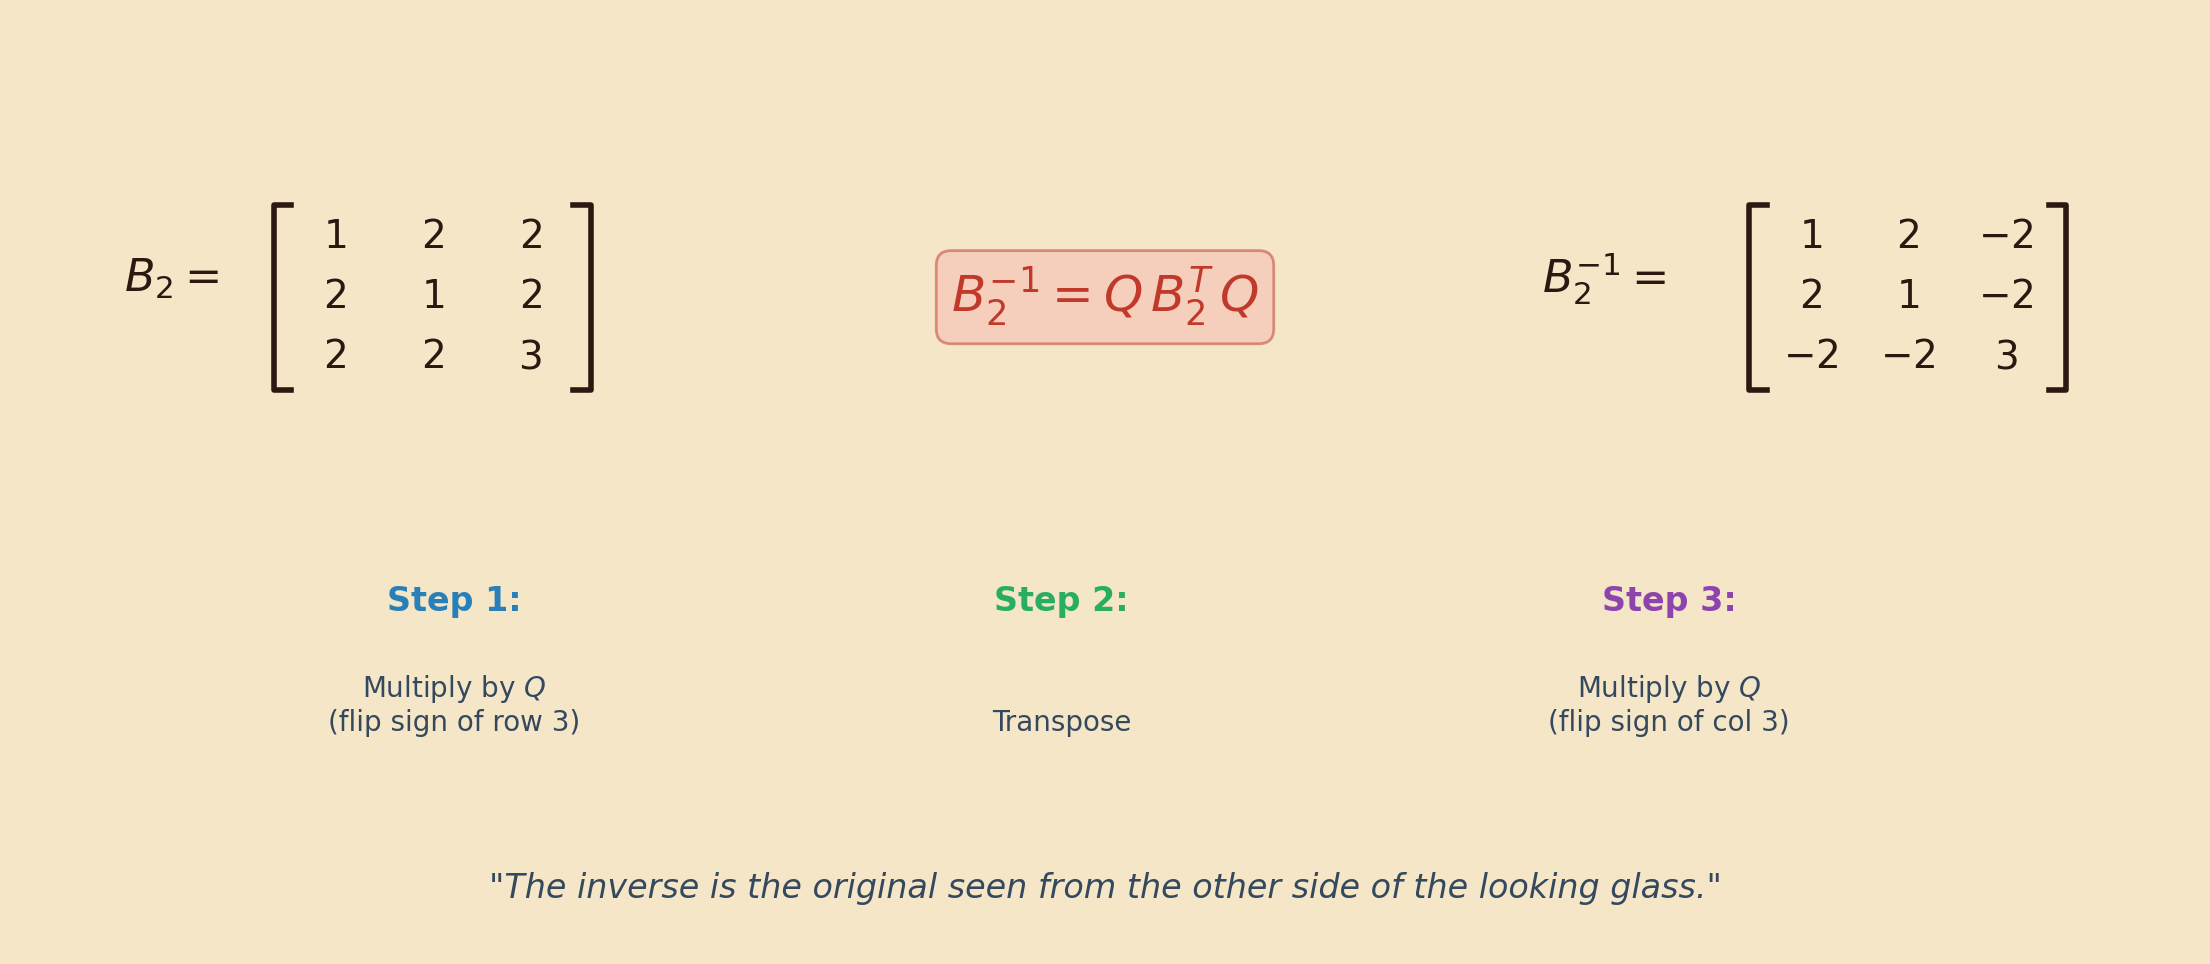
\includegraphics[width=0.82\textwidth]{../Chapter3/images/fig11_lorentz_adjoint.png}
\caption{A side-by-side display of $B_2$ and $B_2^{-1}$. Between them, the Lorentz adjoint formula $B_2^{-1} = \mathbf{Q}\, B_2^\top\, \mathbf{Q}$ is written in an elegant calligraphic font. Arrows show the\ldots}
\end{figure}


\bigskip


\section{Why the Hypotenuse Always Grows (and How Fast)}

Here is a strange claim: once you leave the root of the Berggren tree, you can never return to a smaller hypotenuse by going \textit{deeper}. The tree only grows. But does every branch grow at the same rate, or does one sprint ahead while another ambles?

To answer this, recall the formulas for the hypotenuse of each child. If the parent is $(a, b, c)$, then:

\begin{itemize}
\item **Left branch ($B_1$):** new hypotenuse $= 2a - 2b + 3c$.
\item **Middle branch ($B_2$):** new hypotenuse $= 2a + 2b + 3c$.
\item **Right branch ($B_3$):** new hypotenuse $= -2a + 2b + 3c$.
\end{itemize}
Let us check that each of these exceeds $c$, the parent's hypotenuse.

The \textbf{middle branch} is obvious: $2a + 2b + 3c > 3c > c$ whenever $a, b > 0$. The middle child always has a strictly larger hypotenuse than its parent, by a margin of at least $2a + 2b$.

The \textbf{left branch} requires a moment's thought. We need $2a - 2b + 3c > c$, or equivalently $2a - 2b + 2c > 0$, i.e., $a - b + c > 0$. Since $c > 0$ and $c > b$ (from the Pythagorean equation), we have $c - b > 0$, so $a + (c - b) > 0$. Done.

The \textbf{right branch} is similar: we need $-2a + 2b + 3c > c$, or $-a + b + c > 0$. Since $c > a$ (again from the Pythagorean equation), we have $c - a > 0$, so $b + (c - a) > 0$. Done.

So the hypotenuse \textit{always} increases --- but the middle branch increases fastest. In fact, the middle branch is explosive. Starting from $(3, 4, 5)$ with $c = 5$:

\begin{center}
\begin{tabular}{c c}
\toprule
Level & Middle-branch hypotenuse \\
\midrule
0 & $5$ \\
1 & $29$ \\
2 & $169$ \\
3 & $985$ \\
4 & $5{,}741$ \\
\bottomrule
\end{tabular}
\end{center}

The hypotenuse roughly sextuples at each step. This is not a coincidence --- it is the fingerprint of a linear recurrence, which brings us to one of the loveliest surprises in this chapter.

\begin{figure}[htbp]
\centering
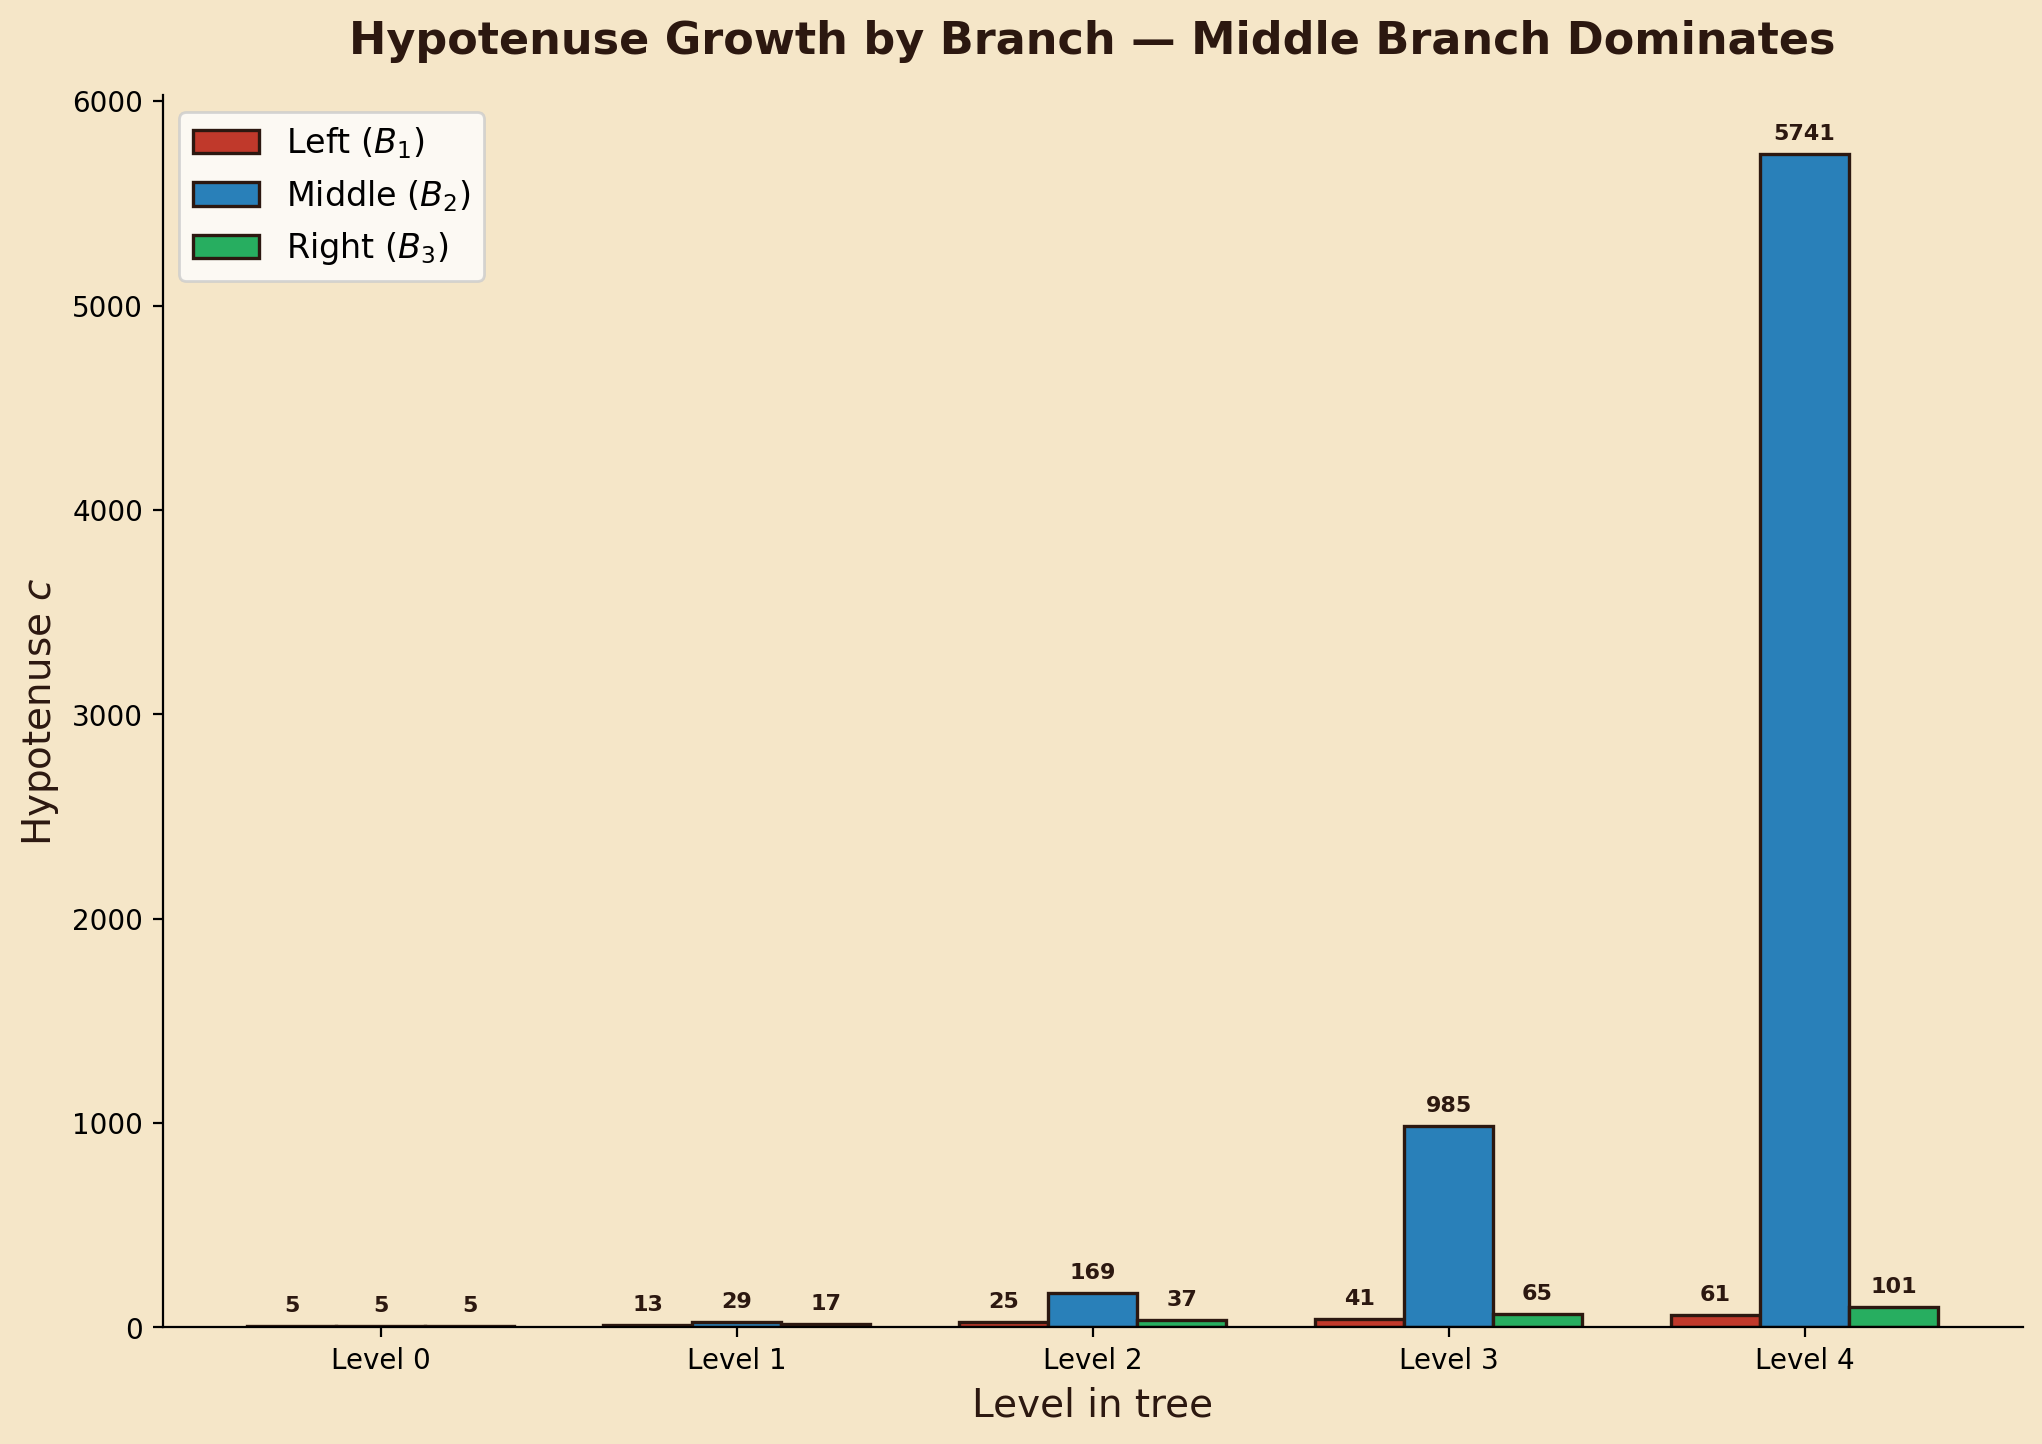
\includegraphics[width=0.82\textwidth]{../Chapter3/images/fig12_hypotenuse_bars.png}
\caption{A bar chart with three groups of bars, one for each branch (Left, Middle, Right), showing the hypotenuses at levels 0 through 4. The Middle branch bars rocket upward exponentially (5, 29, 169, 985,\ldots}
\end{figure}


\bigskip


\section{Chebyshev's Secret Recurrence}

The middle branch of the Berggren tree produces the hypotenuse sequence:

\[
5, \; 29, \; 169, \; 985, \; 5741, \; \ldots
\]

Stare at these numbers. Can you spot the pattern? Here is a hint:

\[
169 = 6 \times 29 - 5.
\]
\[
985 = 6 \times 169 - 29.
\]
\[
5741 = 6 \times 985 - 169.
\]

The pattern is a \textit{linear recurrence}:

\[
c_{n+1} = 6\, c_n - c_{n-1},
\]

with initial values $c_0 = 5$ and $c_1 = 29$. Each term is six times its predecessor minus the term before that. Verify:

\[
c_2 = 6 \cdot 29 - 5 = 174 - 5 = 169. \quad \checkmark
\]
\[
c_3 = 6 \cdot 169 - 29 = 1014 - 29 = 985. \quad \checkmark
\]
\[
c_4 = 6 \cdot 985 - 169 = 5910 - 169 = 5741. \quad \checkmark
\]

Beautiful. But why does this recurrence appear?

The answer lies in the theory of matrix powers. The middle-branch matrix $B_2$ is a $3 \times 3$ matrix, and the Cayley--Hamilton theorem guarantees that it satisfies its own characteristic polynomial. This polynomial, being cubic, means that the third power of $B_2$ can be expressed as a linear combination of $B_2^2$, $B_2$, and the identity. When you project this relation onto the hypotenuse coordinate, the three-term matrix relation reduces to a two-term scalar recurrence --- and the coefficient $6$ emerges from the trace and other invariants of $B_2$.
\index{Hamilton, William Rowan}

The name "Chebyshev" enters because recurrences of the form $c_{n+1} = \alpha \, c_n - c_{n-1}$ are intimately connected to \textbf{Chebyshev polynomials of the first kind}. These are the polynomials $T_n(\cos\theta) = \cos(n\theta)$ --- a family of functions that arise whenever one studies powers of $2 \times 2$ matrices, trigonometric identities, or best approximation in function spaces. The connection is not superficial: the eigenvalues of $B_2$, restricted to the relevant two-dimensional invariant subspace, generate a recurrence that is a Chebyshev polynomial in disguise.

And notice something tantalizing: $c_2 = 169 = 13^2$. The second term in the middle-branch hypotenuse sequence is a perfect square! This is not an accident, and it connects back to our opening puzzle: perfect-square hypotenuses lead to especially clean factorizations via the difference-of-squares trick. The middle branch is not merely the fastest-growing branch --- it is also the one most richly endowed with algebraic structure.

Pafnuty Lvovich Chebyshev (1821--1894) would have appreciated this connection. The great Russian mathematician worked at the intersection of number theory, probability, and approximation theory. His polynomials were born from a question about best approximation --- how closely can a polynomial of degree $n$ approximate a given function? --- but they have infiltrated an astonishing range of mathematics, from mechanical linkage design to signal processing to, as we now see, the internal recurrences of the Berggren tree.

\begin{figure}[htbp]
\centering
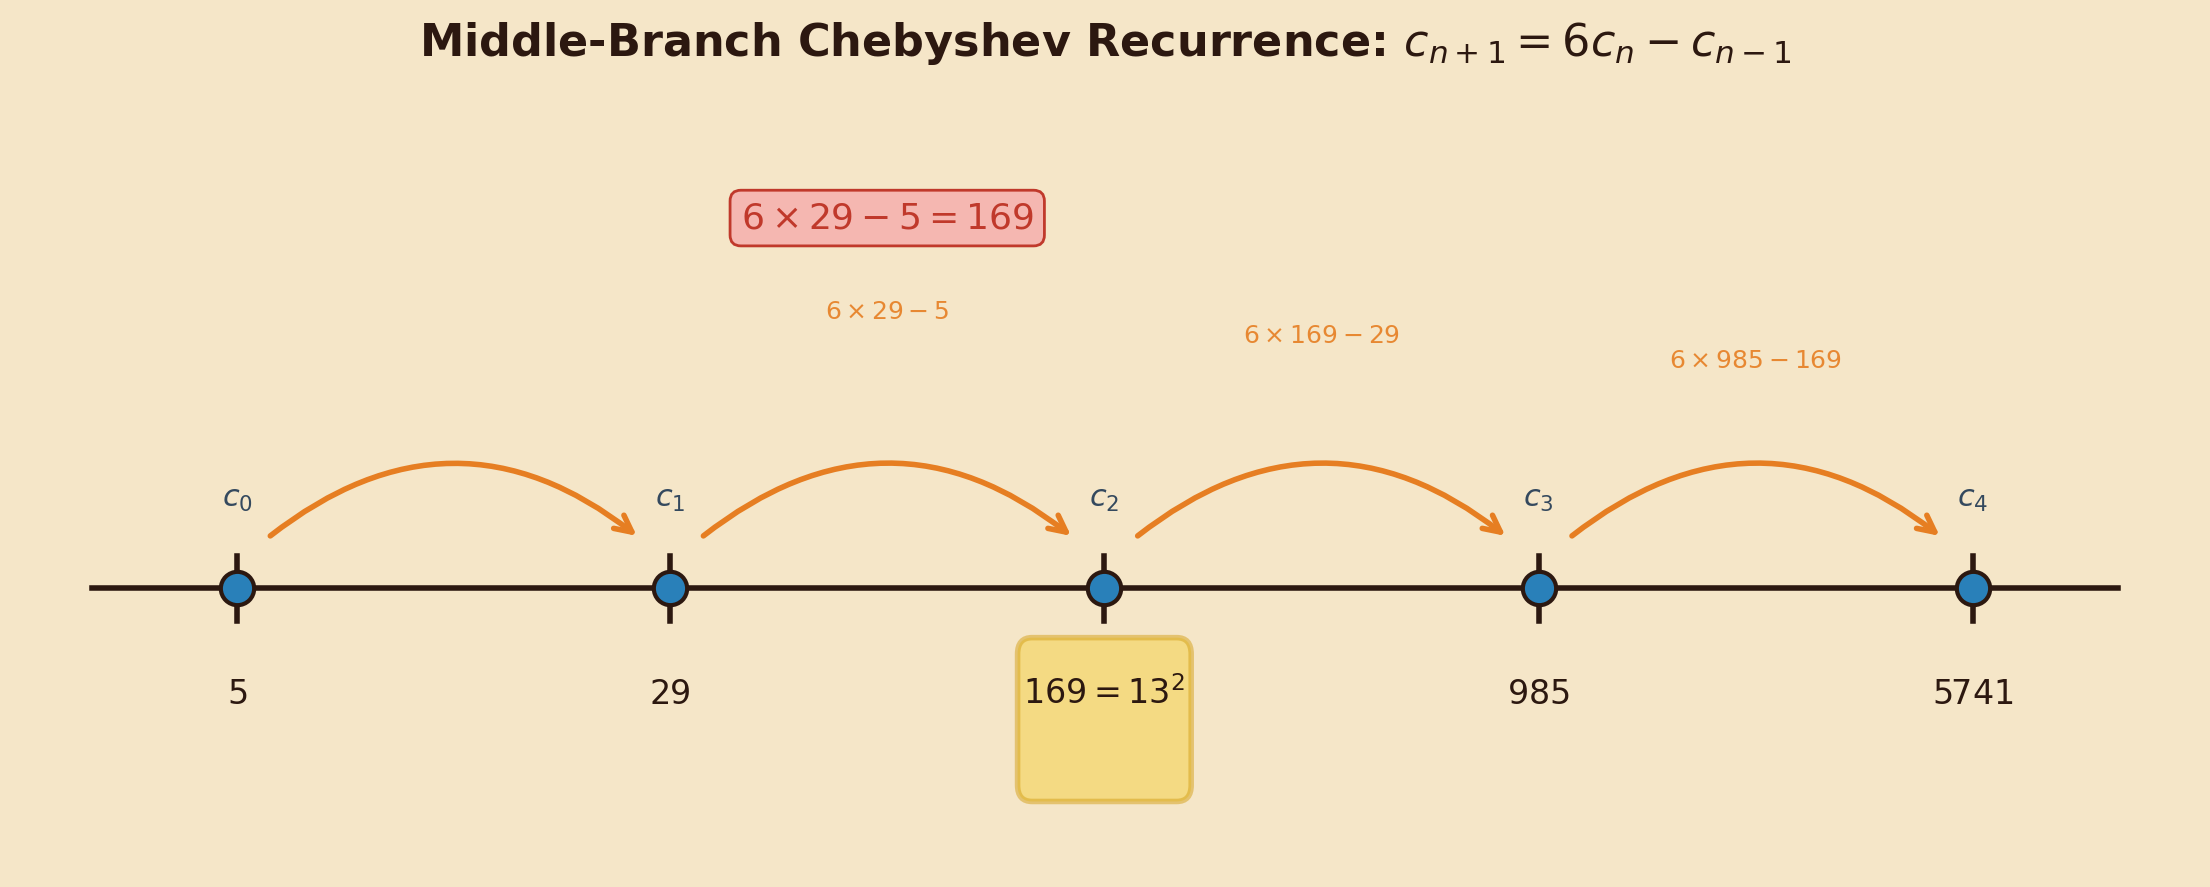
\includegraphics[width=0.82\textwidth]{../Chapter3/images/fig13_chebyshev_line.png}
\caption{A number line running horizontally across the page, with the middle-branch hypotenuses $5, 29, 169, 985, 5741$ marked at their positions (not to scale --- logarithmic spacing). Curved arrows arc above\ldots}
\end{figure}


\bigskip


\section{No Two Branches Bear the Same Fruit}

In a well-designed filing system, no document should appear in two drawers at once. The Berggren tree is nature's filing system for Pythagorean triples. Can two different branches --- say, the left and middle children of the same parent --- ever produce the same triple?

Let us see why the answer is \textit{never}, at least locally.

**Claim 1: $B_1$ and $B_2$ always produce distinct hypotenuses.** The left-branch hypotenuse is $2a - 2b + 3c$, and the middle-branch hypotenuse is $2a + 2b + 3c$. If these were equal, we would need $4b = 0$, i.e., $b = 0$. But for a genuine Pythagorean triple with all positive entries, $b > 0$. So the hypotenuses differ, and therefore the triples differ.

**Claim 2: $B_1$ and $B_3$ always produce distinct hypotenuses (when $a \neq b$).** The left-branch hypotenuse is $2a - 2b + 3c$, and the right-branch hypotenuse is $-2a + 2b + 3c$. Equality would require $4a - 4b = 0$, i.e., $a = b$. For a primitive Pythagorean triple, one leg is always odd and the other is always even (a classical fact from Euclid's parametrization), so $a \neq b$ --- and the hypotenuses are distinct.

**Claim 3: $B_2$ and $B_3$ always produce distinct hypotenuses.** The middle-branch hypotenuse is $2a + 2b + 3c$, and the right-branch hypotenuse is $-2a + 2b + 3c$. Equality requires $4a = 0$, i.e., $a = 0$. Impossible for a positive triple.

In every case, the three children of any node have three different hypotenuses. Since no two children at the same level share a hypotenuse, no two children are the same triple. This "local disjointness" is the engine behind the deeper global theorem, attributed to Berggren and Hall:

\begin{quote}
\itshape \textbf{Theorem (Berggren--Hall).} Every primitive Pythagorean triple appears exactly once in the Berggren tree.
\end{quote}

The proof of the global theorem --- that no triple appears anywhere in the tree more than once, even in completely different branches at different depths --- requires more machinery than we have assembled here. But the local disjointness gives you the essential flavor: the tree is intrinsically incapable of repeating itself, because each branching step produces three genuinely different outputs.

\begin{figure}[htbp]
\centering
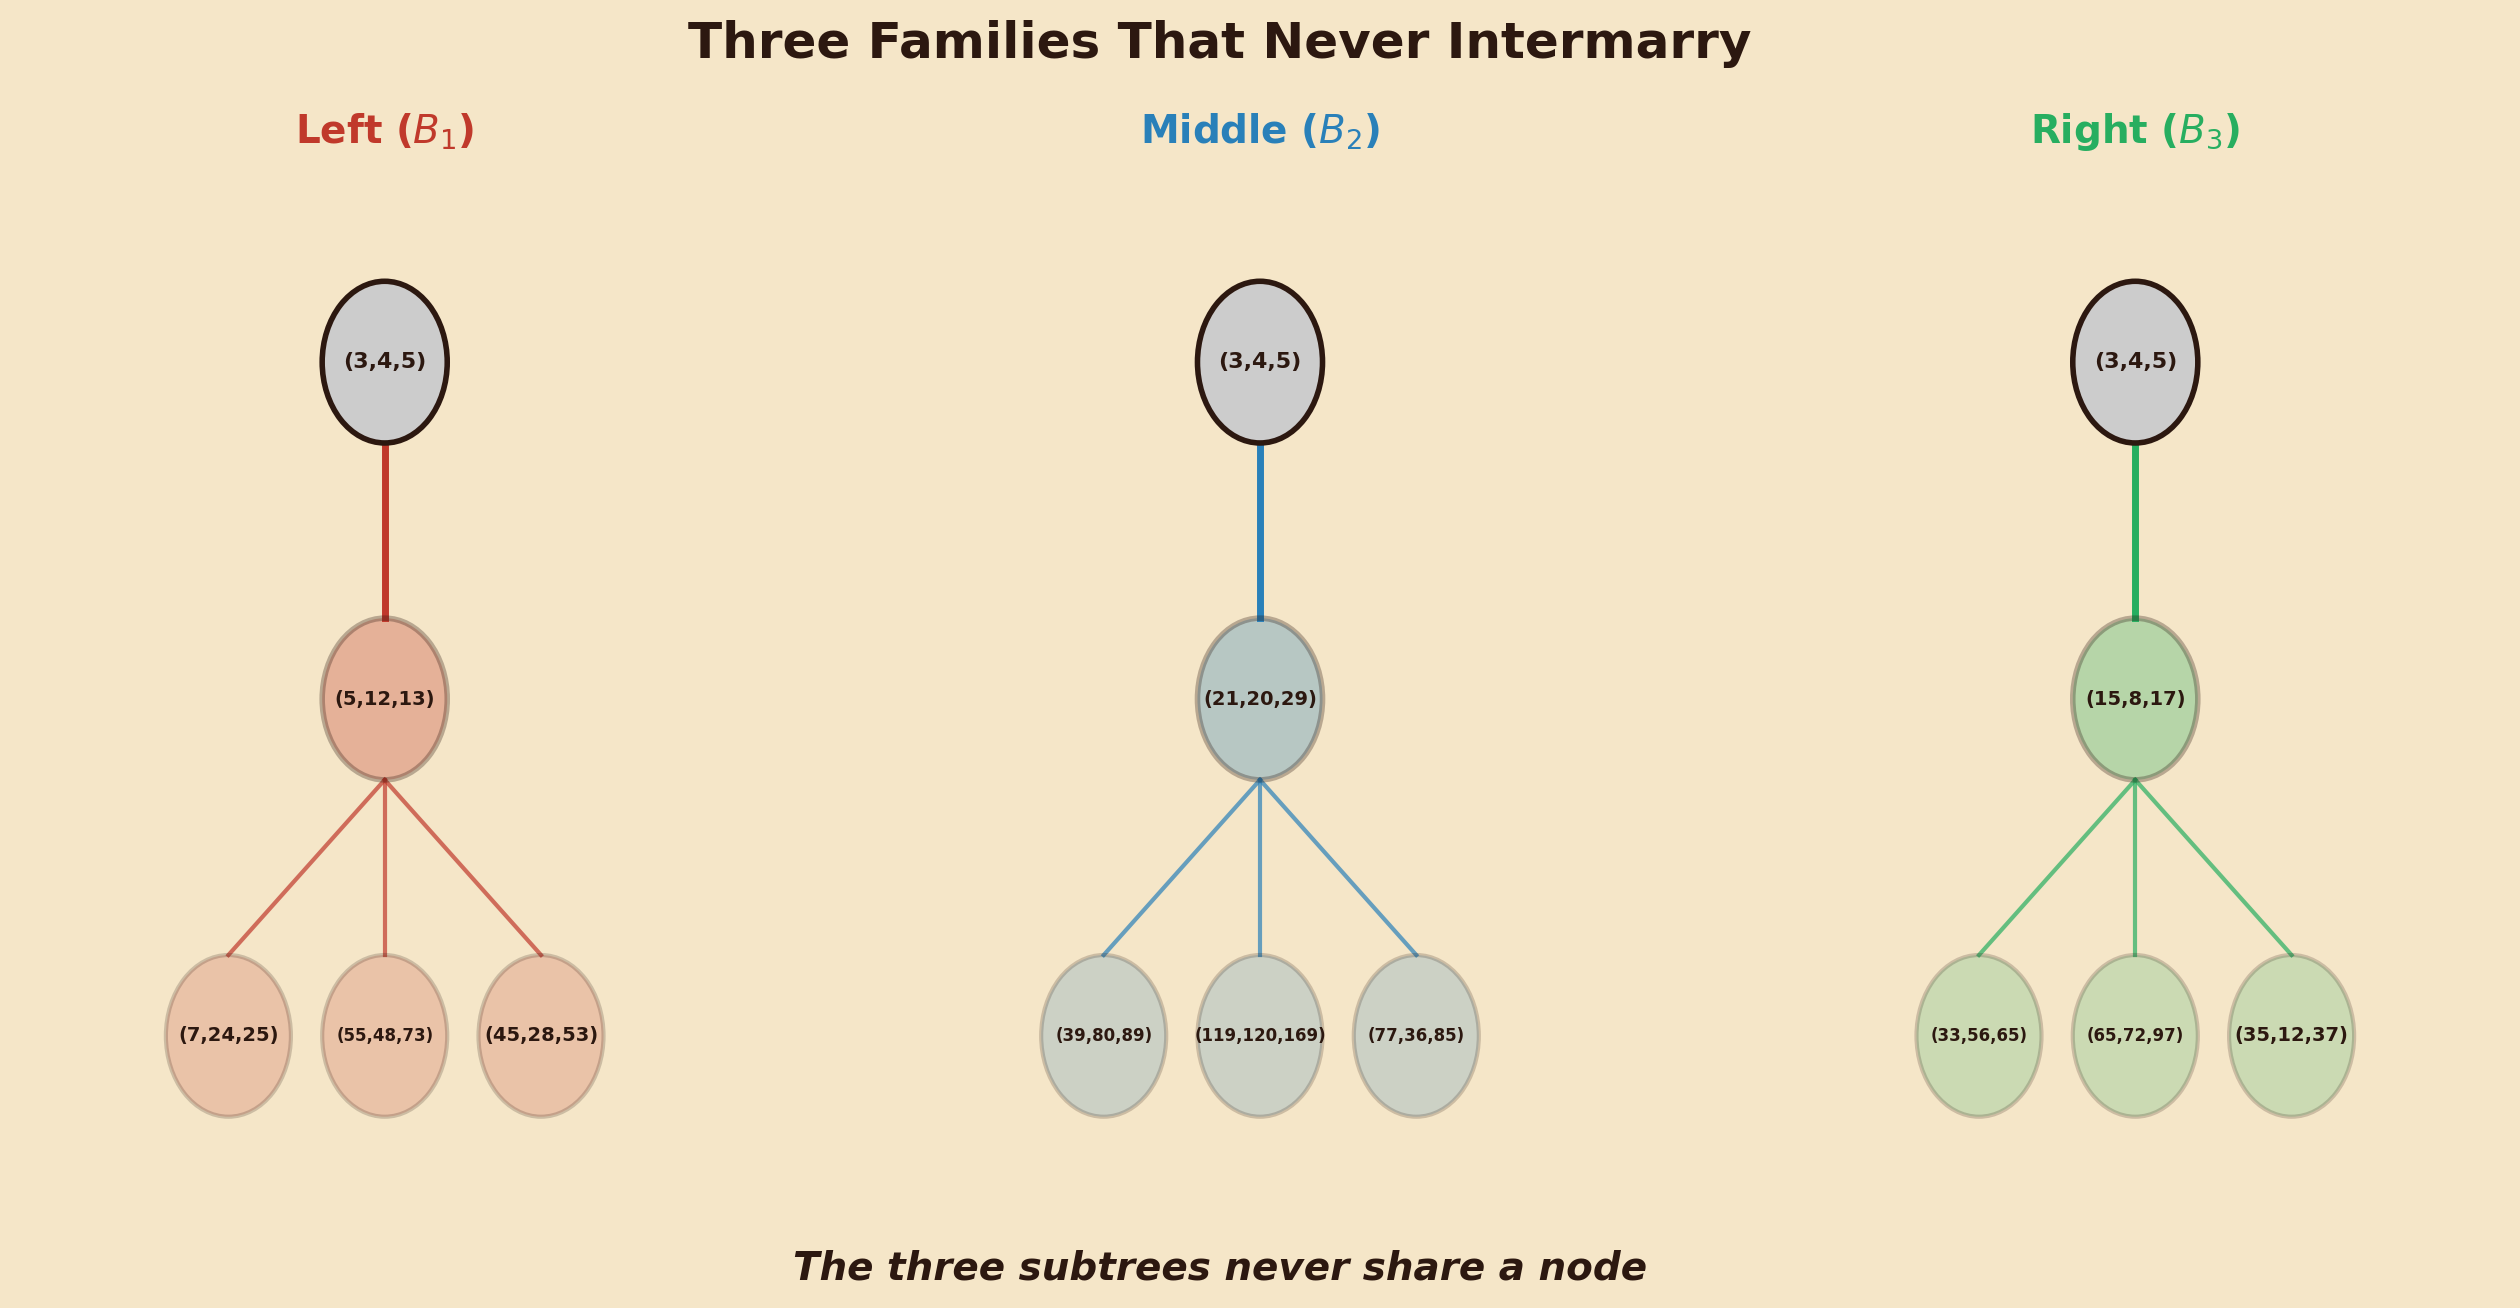
\includegraphics[width=0.82\textwidth]{../Chapter3/images/fig14_three_subtrees.png}
\caption{Three subtrees of the Berggren tree drawn side by side, one for each branch (Left in red, Middle in blue, Right in green). All three are rooted at the same parent node $(3, 4, 5)$, shown in grey at\ldots}
\end{figure}


\bigskip


\section{Cracking Numbers on the Light Cone}

At last, we arrive at the punchline.

We began this chapter with a parlour trick: factoring $441$ using a Pythagorean triple. Now let us elevate the trick to a method.

\textbf{The Setup.} You are given a composite number $N$ and asked to find a nontrivial factor --- some $d$ with $1 < d < N$ that divides $N$. (This is the central problem of computational number theory, and the security of the internet depends on its difficulty for large $N$.) Here is the Pythagorean approach.

\textbf{Step 1.} Find a Pythagorean triple $(a, b, c)$ with $a = N$ --- or, more generally, with $a$ sharing a nontrivial factor with $N$. The Berggren tree provides a structured source of triples.

\textbf{Step 2.} Compute $c - b$. By the difference-of-squares identity:

\[
(c - b)(c + b) = a^2 = N^2.
\]

\textbf{Step 3.} Compute $d = \gcd(c - b, \, N)$. If $1 < d < N$, you have found a nontrivial factor. Done.

Why does this work? Because $c - b$ divides $N^2$, so $\gcd(c - b, N)$ divides $N$. The only question is whether the GCD is trivial (equal to $1$ or $N$) or nontrivial. In many cases, it is nontrivial --- and the factor pops out with no trial division, no sieving, and no sophisticated prime-detection machinery. Just one subtraction and one GCD.

Let us state this precisely.

\textbf{Theorem (GCD Factoring via Pythagorean Triples).} If $a^2 + b^2 = c^2$ with $a > 1$, and if $d = \gcd(c - b, \, a)$ satisfies $1 < d < |a|$, then $d$ is a nontrivial divisor of $a$.

The proof is almost trivial. We have $(c - b)(c + b) = a^2$, so $c - b$ divides $a^2$. Therefore $\gcd(c - b, a)$ divides $a$. The theorem simply asserts that this GCD is neither $1$ nor $|a|$ --- and that is a condition we can check.

\textbf{Worked example.} Take $N = 21$ and the triple $(21, 20, 29)$.

\[
c - b = 29 - 20 = 9.
\]
\[
\gcd(9, 21) = 3.
\]

Since $1 < 3 < 21$, we have discovered that $3$ divides $21$. And $21 / 3 = 7$. Factorization complete: $21 = 3 \times 7$.

Let us try another. Take $N = 65$ and the triple $(33, 56, 65)$.

Wait --- here $a = 33$, not $65$. We need $N$ to be a \textit{leg}, not the hypotenuse. But the Berggren tree can also help us find triples with $c = N$ or with $a$ or $b$ sharing factors with $N$. The method is flexible.

Let us instead try the triple $(65, 72, 97)$, where $a = 65$.

\[
c - b = 97 - 72 = 25.
\]
\[
\gcd(25, 65) = 5.
\]

Since $1 < 5 < 65$, we have found a factor: $65 = 5 \times 13$.

Not every triple yields a nontrivial GCD. For the triple $(3, 4, 5)$:

\[
c - b = 5 - 4 = 1.
\]
\[
\gcd(1, 3) = 1.
\]

Trivial --- no factor revealed. This makes sense: $3$ is prime, so no amount of algebraic cleverness can split it into smaller factors. The method works best when $a$ is composite and the triple's geometry happens to align with the factorization.

\begin{figure}[htbp]
\centering
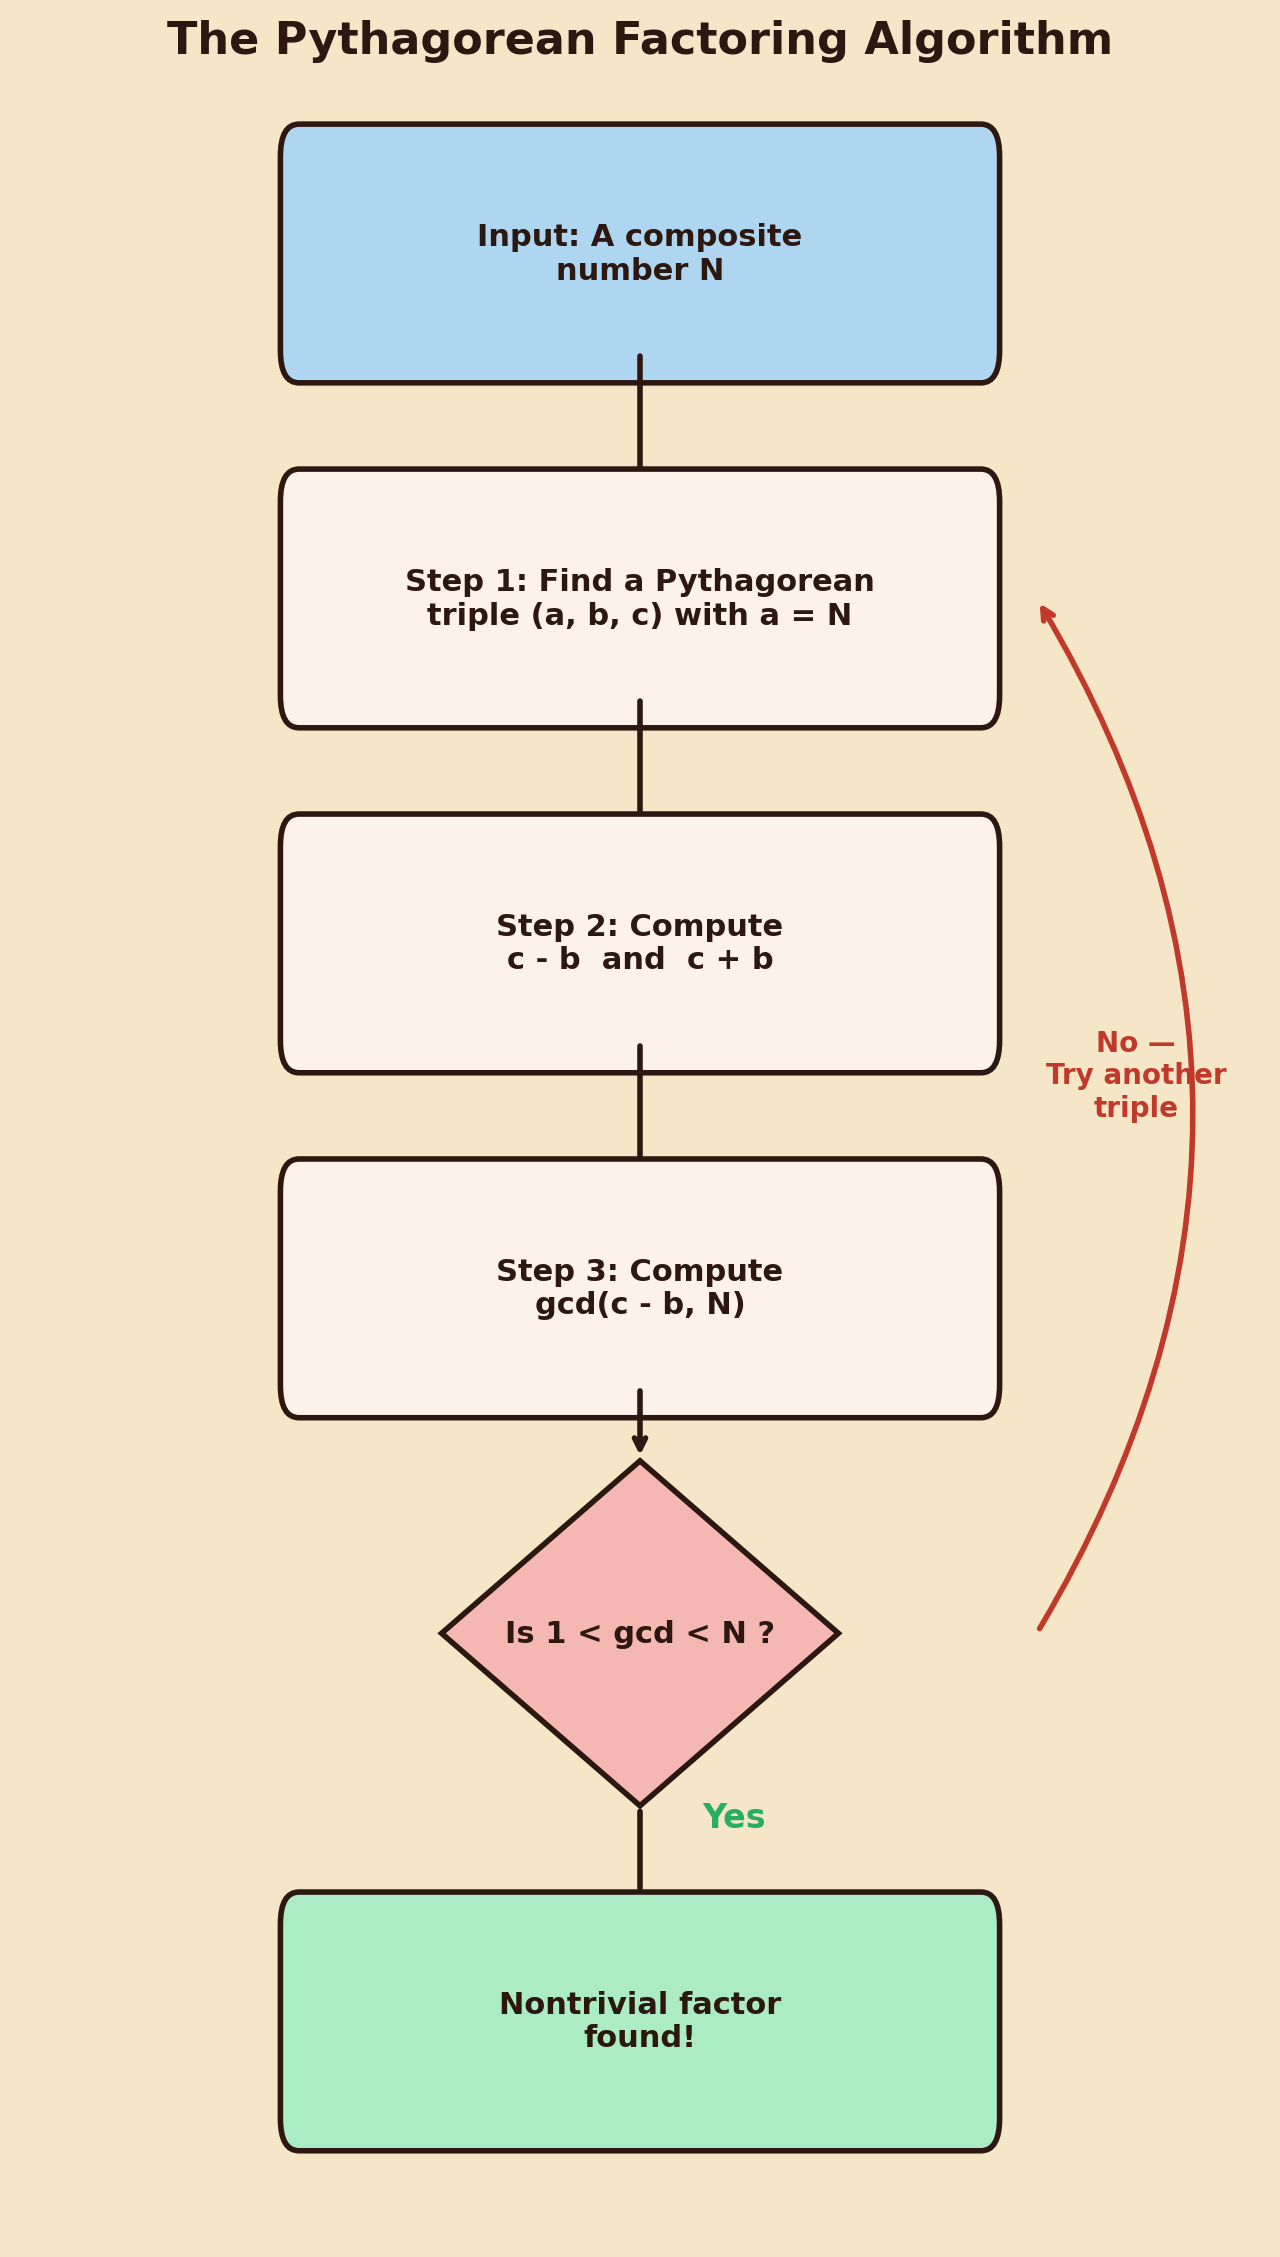
\includegraphics[width=0.82\textwidth]{../Chapter3/images/fig15_factoring_flowchart.png}
\caption{A flowchart-style diagram, elegant and vertical. \textbf{Input box} at the top: "A composite number $N$." \textbf{Arrow down} to \textbf{Step 1}: "Find a Pythagorean triple $(a, b, c)$ with $a = N$."\ldots}
\end{figure}

\begin{figure}[htbp]
\centering
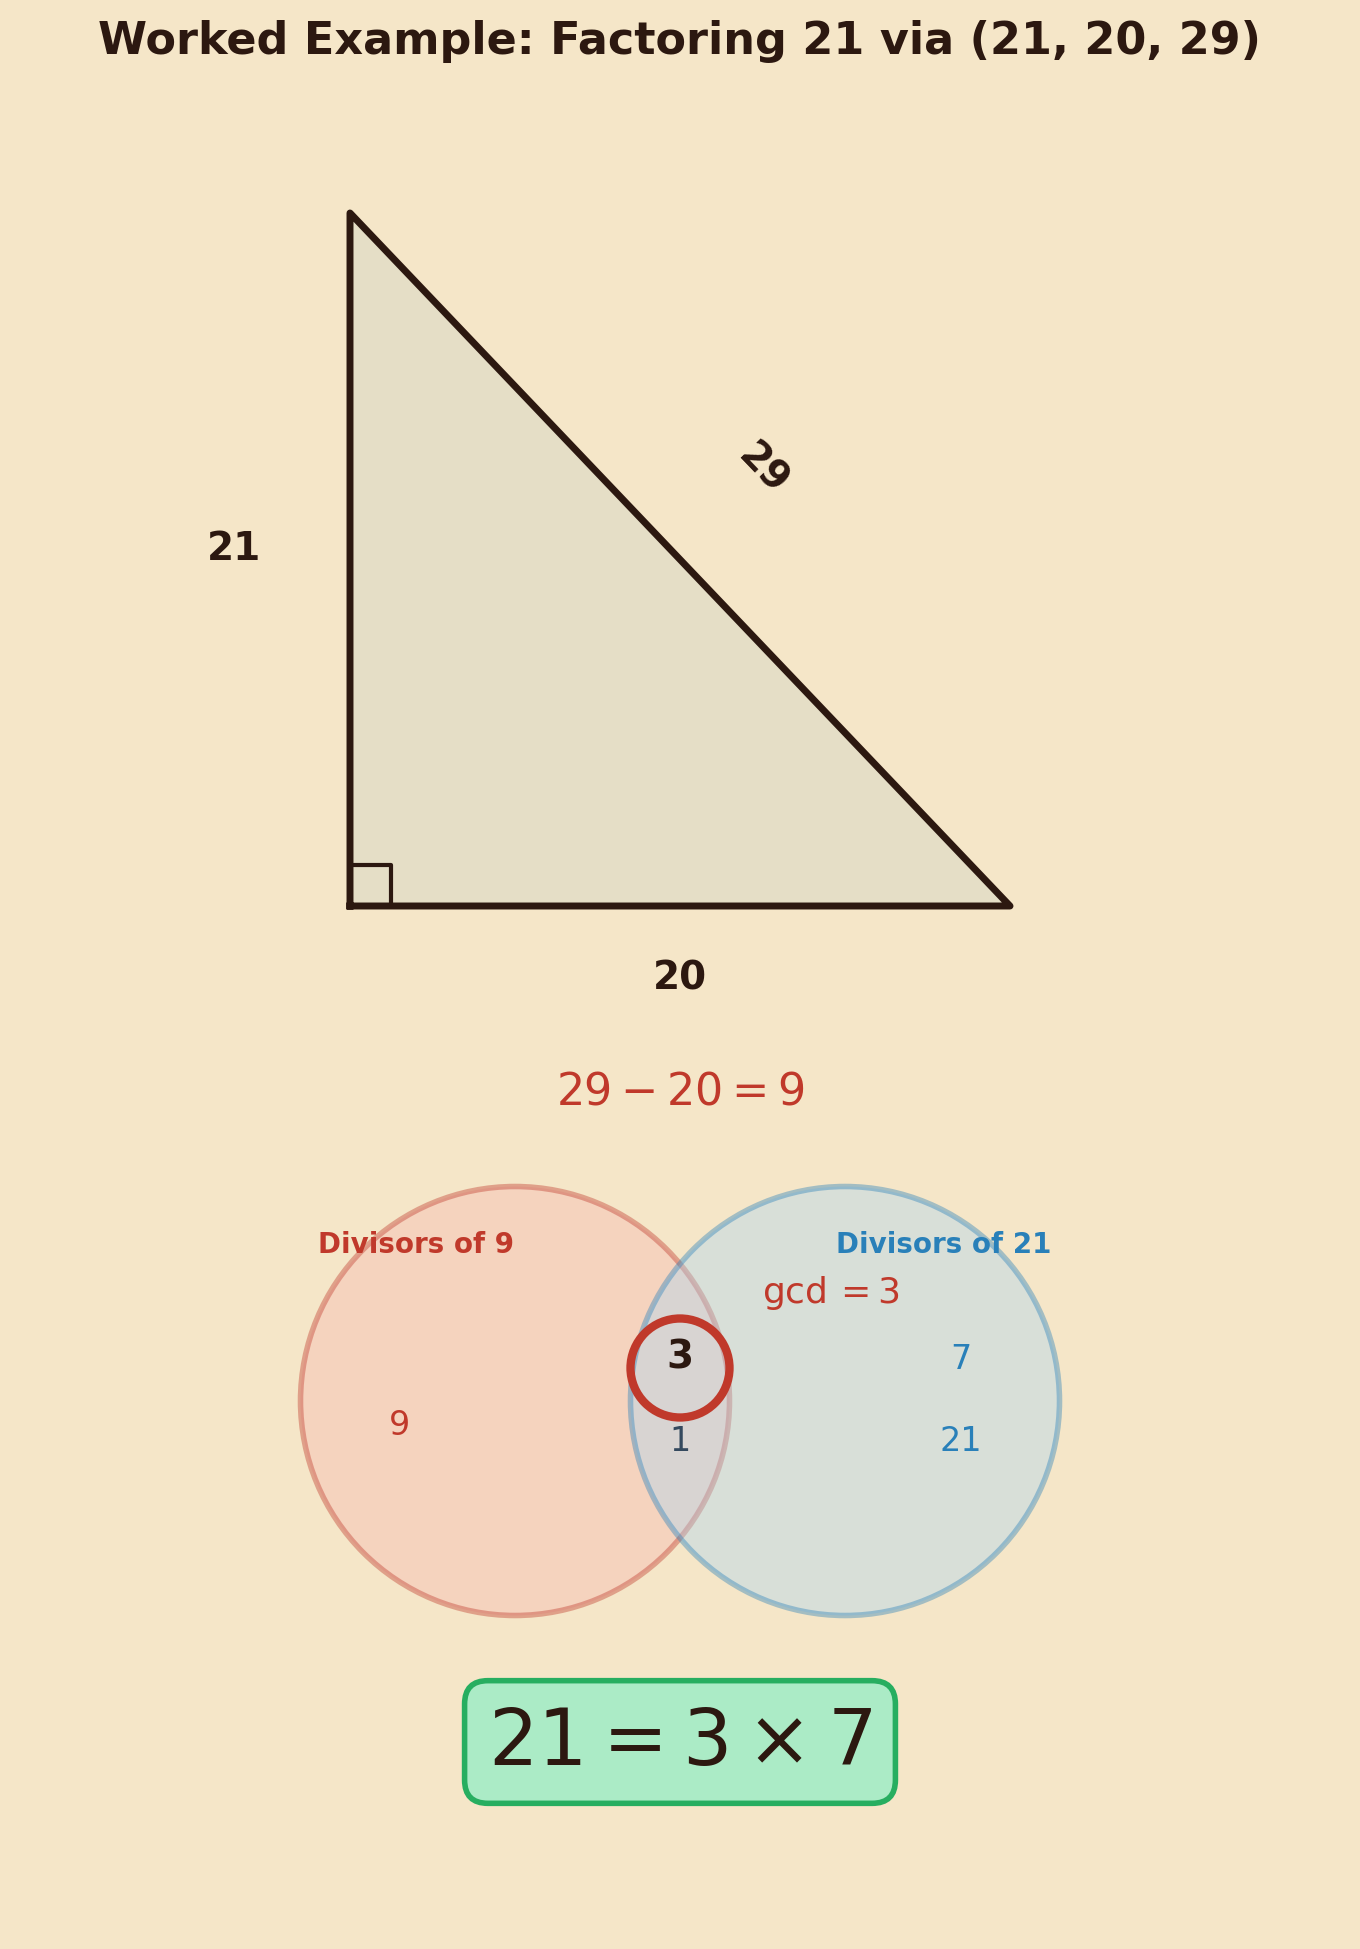
\includegraphics[width=0.82\textwidth]{../Chapter3/images/fig16_worked_example.png}
\caption{The specific worked example for $(21, 20, 29)$, laid out as a visual "proof without words." At the top, the right triangle with sides $21$, $20$, $29$. Below it, a horizontal arrow from $29$ to $20$\ldots}
\end{figure}

The connection to Fermat's factoring method is now clear. Fermat's approach, dating to the 1640s, searches for representations $N = x^2 - y^2 = (x - y)(x + y)$. The Pythagorean approach provides these representations \textit{automatically} from the geometry of right triangles: every Pythagorean triple gives a free difference of squares, and the Berggren tree gives a systematic way to generate candidates. The modern quadratic sieve and number field sieve --- the algorithms that actually break large numbers in practice --- are, at a deep level, industrialized descendants of the same difference-of-squares principle. They generate many relations of the form $x^2 \equiv y^2 \pmod{N}$ and combine them using linear algebra over $\mathbb{F}_2$ to find a factor. The Berggren tree is the artisanal workshop; the quadratic sieve is the factory.


\bigskip


\section{Epilogue: Through the Wormhole}

We began with a broken square and ended with a factoring machine powered by the symmetries of spacetime. Let us take one last look at the landscape before moving on.

The chapter's journey followed a single thread, but the thread wound through five very different territories:

\begin{enumerate}
\item \textbf{The Ancient Identity.} The humble equation $(c - b)(c + b) = a^2$ --- a one-line consequence of the Pythagorean theorem --- turned out to be a factoring engine. (?1)
\item \textbf{The Berggren Tree.} Three $3 \times 3$ matrices, discovered by a Swedish schoolteacher in 1934, generate every primitive Pythagorean triple from the single seed $(3, 4, 5)$. (?2)
\item \textbf{The Lorentz Connection.} The Berggren matrices are integer Lorentz transformations --- they preserve the quadratic form $Q(a, b, c) = a^2 + b^2 - c^2$, which is the equation of a light cone in Minkowski spacetime. Pythagorean triples are null vectors, and the tree lives on the surface of the cone. (?3--?4)
\item \textbf{Paths and Shortcuts.} Every triple has a unique address in the tree, and the address can be traversed in logarithmic time using repeated squaring. Inverse matrices --- computed via the Lorentz adjoint --- let you climb back up from any node to the root. (?5--?7)
\item \textbf{Structure and Growth.} The hypotenuse always increases as you descend, with the middle branch growing fastest (governed by a Chebyshev recurrence). No two branches ever produce the same triple. And the difference-of-squares identity, combined with a GCD computation, turns any triple into a factoring tool. (?8--?11)
\end{enumerate}
The deepest surprise, to my mind, is the Lorentz connection. There is no a priori reason why the arithmetic of right triangles --- a subject as old as civilization --- should have anything to do with the geometry of spacetime --- a subject born in 1905. And yet the Berggren matrices sit squarely in the integer Lorentz group, and the invariant that propagates the Pythagorean property down the tree is precisely the invariant that propagates the speed of light through Einstein's universe. The amateur's delight in a $3$-$4$-$5$ triangle and the physicist's delight in Lorentz invariance turn out to be the same delight, viewed from different ends of a very long telescope.

In the next chapter, we will shift perspective entirely. If the Berggren tree generates all primitive Pythagorean triples by matrix multiplication, can we understand the same triples through a completely different lens --- the lens of \textit{Gaussian integers}, where the Pythagorean equation dissolves into the norm of a complex number? The answer will bring together three seemingly independent roads --- parametric, geometric, and algebraic --- and reveal that they converge at a single crossroads.
\index{Gaussian integers}
\index{complex numbers}

But that is a story for another day.

\begin{figure}[htbp]
\centering
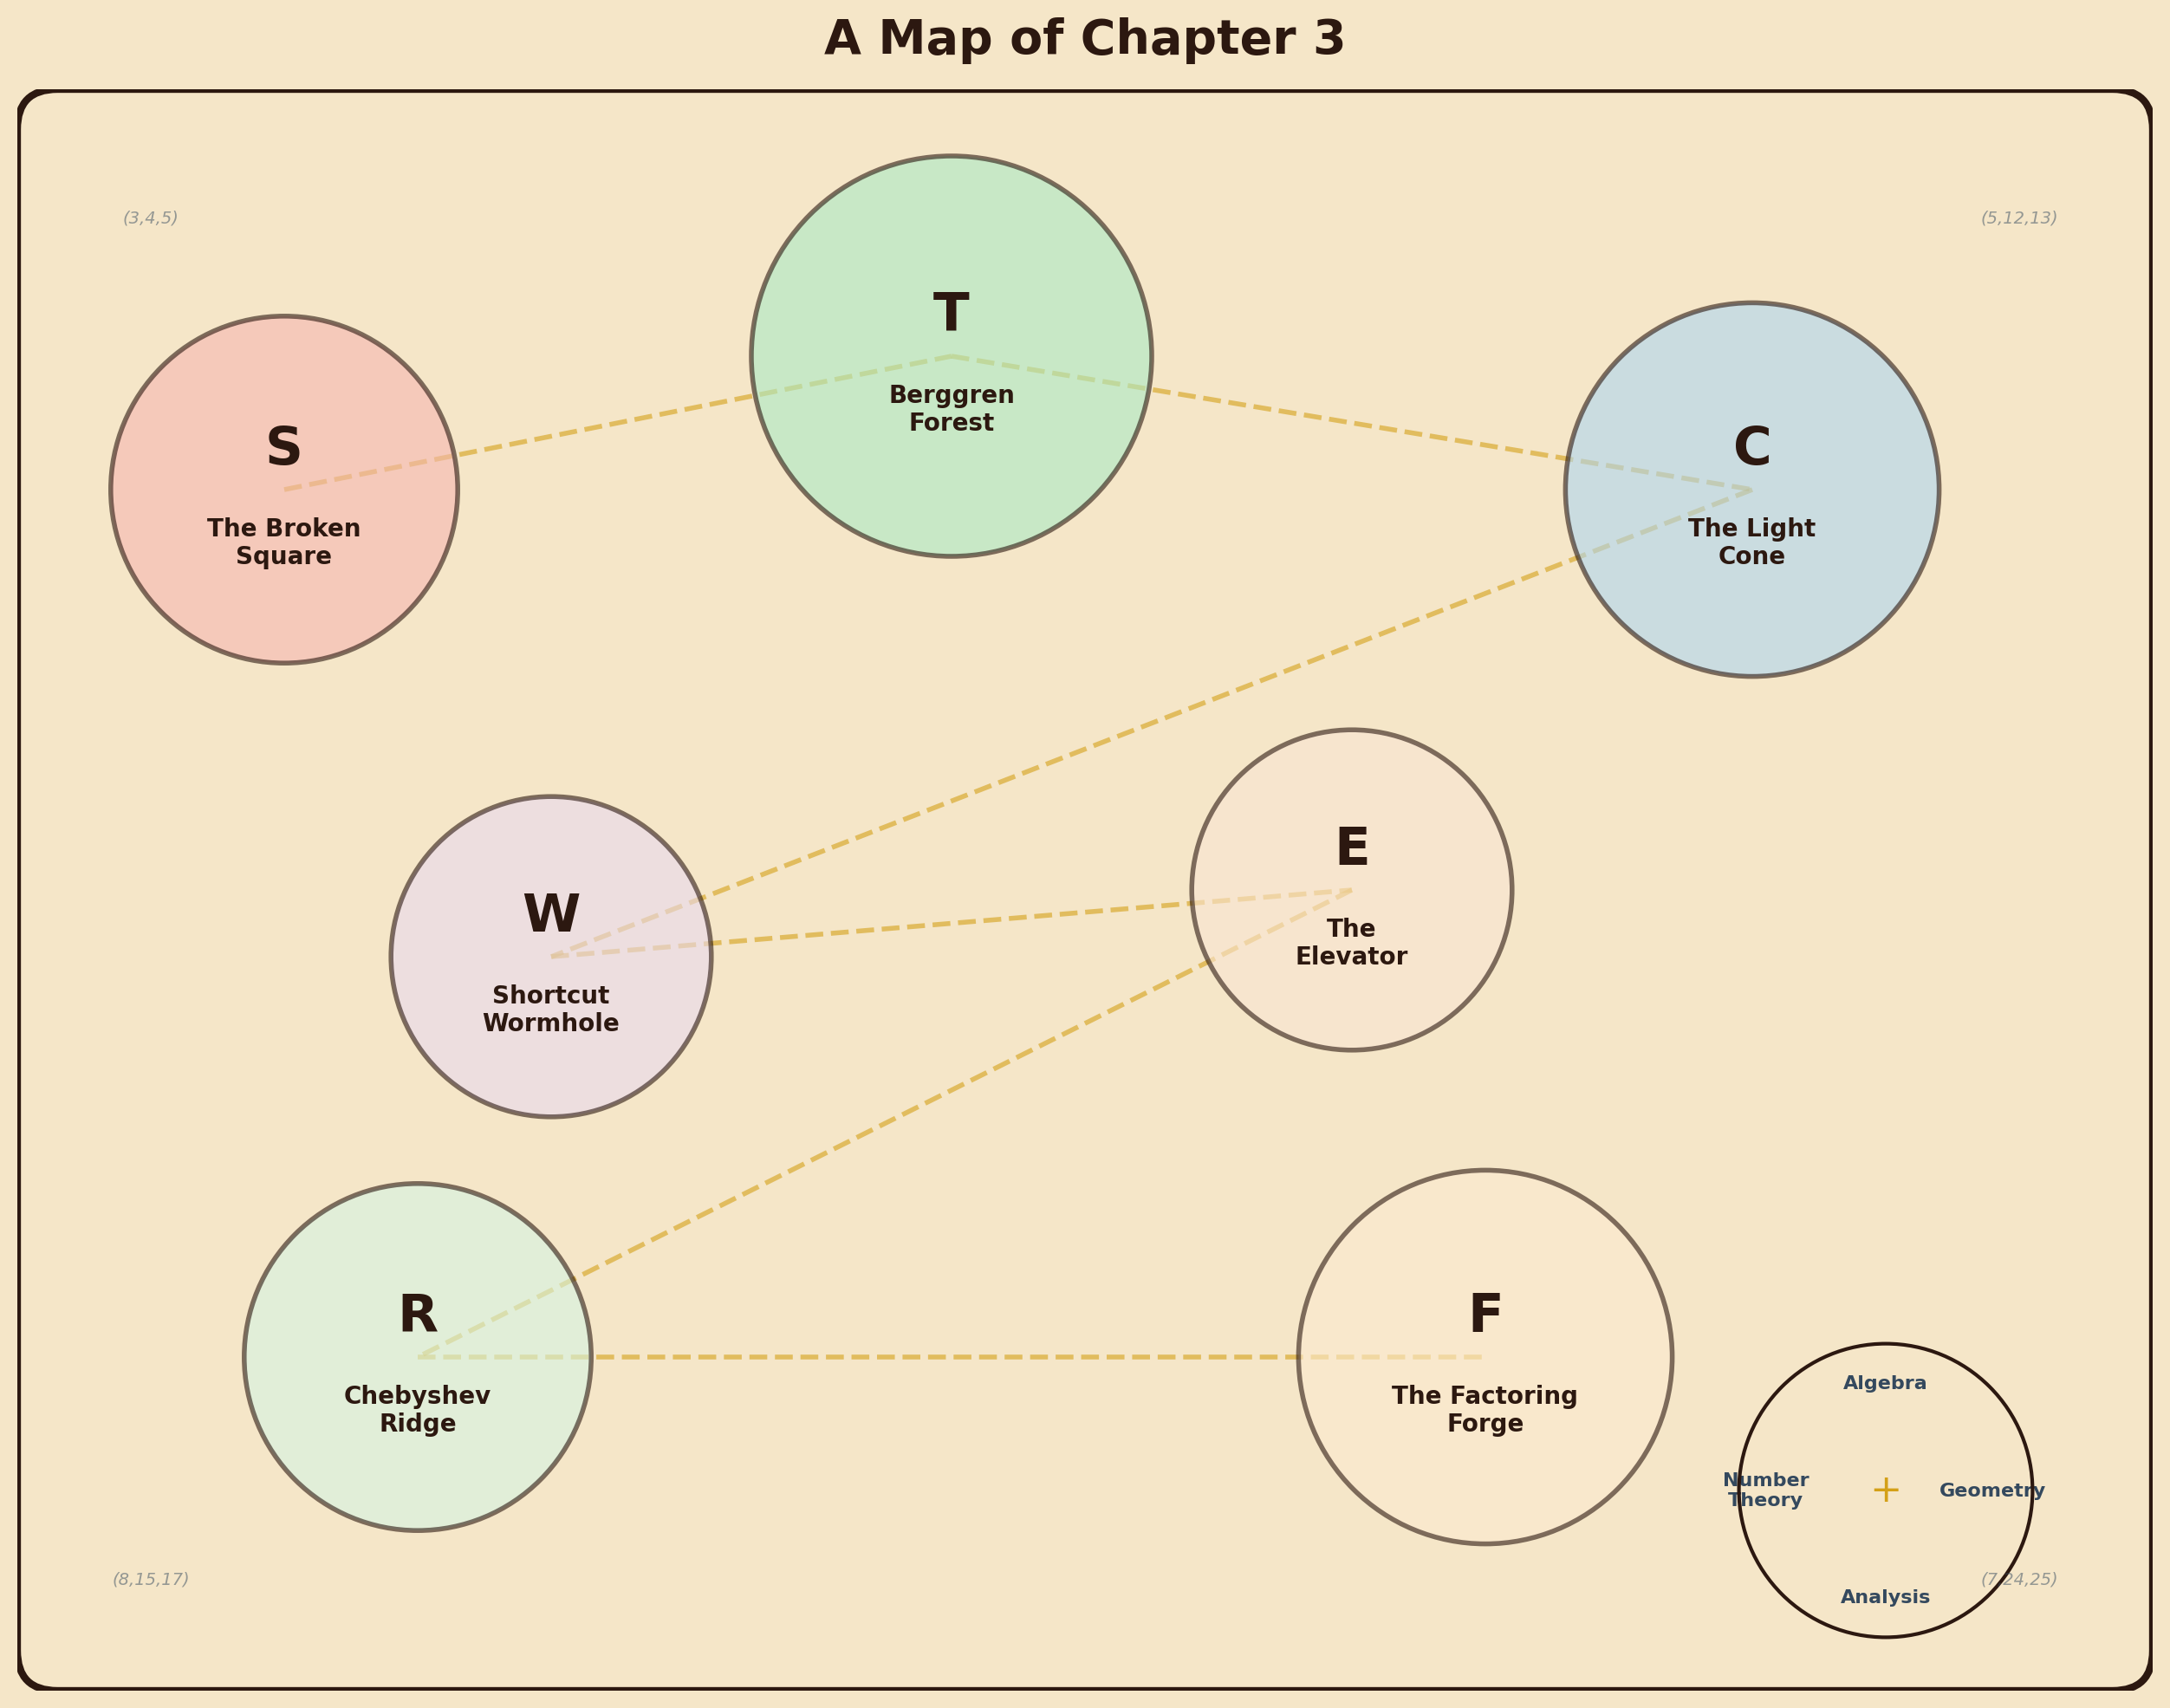
\includegraphics[width=0.82\textwidth]{../Chapter3/images/fig17_concept_map.png}
\caption{A full-page "map" of the chapter's conceptual landscape, drawn in the style of a medieval mappa mundi or a fantasy-novel treasure map. The map contains labeled regions: "The Broken Square" (a cracked\ldots}
\end{figure}


\bigskip


\subsection*{Puzzles for the Reader}

\begin{quote}
\itshape \textbf{Puzzle 1.} The triple $(8, 15, 17)$ is primitive and Pythagorean. Compute $c - b$ and $\gcd(c - b, a)$. Does the GCD reveal a nontrivial factor of $8$?
\end{quote}

\begin{quote}
\itshape \textbf{Puzzle 2.} Find the address of the triple $(7, 24, 25)$ in the Berggren tree by ascending from $(7, 24, 25)$ to the root using inverse matrices. (Hint: try each $B_i^{-1}$ at each step and check which one gives all-positive entries.)
\end{quote}

\begin{quote}
\itshape \textbf{Puzzle 3.} Verify the Chebyshev recurrence $c_{n+1} = 6c_n - c_{n-1}$ for the \textit{legs} of the middle branch, not just the hypotenuses. Do the $a$-values and $b$-values of the middle branch satisfy the same recurrence?
\end{quote}

\begin{quote}
\itshape \textbf{Puzzle 4.} Compute $B_2^2$ explicitly and verify that it sends $(3, 4, 5)$ to $(119, 120, 169)$. Then verify that $169 = 13^2$, and use the difference-of-squares trick to factor the leg $a = 119$.
\end{quote}

\begin{quote}
\itshape \textbf{Puzzle 5.} The Lorentz adjoint formula says $B_i^{-1} = \mathbf{Q} B_i^\top \mathbf{Q}$. Verify this for $B_3$ by computing both sides explicitly.
\end{quote}

\begin{quote}
\itshape \textbf{Puzzle 6.} How many matrix multiplications does it take to compute $B_2^{64}$ by repeated squaring? How about $B_2^{100}$?
\end{quote}

